% Compile with XeLaTeX, three times (or run build.ps1). Entry point for Overleaf: main.tex.
\documentclass[12pt,a4paper,oneside]{report}
\usepackage[margin=2.5cm,headheight=16pt]{geometry}
\usepackage{fontspec}
\IfFontExistsTF{Times New Roman}{\setmainfont{Times New Roman}}{\setmainfont{TeX Gyre Termes}}
\IfFontExistsTF{Arial}{\setsansfont{Arial}}{\setsansfont{TeX Gyre Heros}}
\IfFontExistsTF{Consolas}{\setmonofont{Consolas}[Scale=0.85]}{\setmonofont{DejaVu Sans Mono}[Scale=0.85]}
\usepackage{amsmath,amssymb,graphicx,xcolor,array,booktabs,longtable,tabularx}
\usepackage{tikz}
\usetikzlibrary{arrows.meta,positioning,shapes.geometric,fit,backgrounds,calc}
\usepackage{fancyhdr,titlesec,setspace,enumitem,float,fancyvrb,etoolbox,needspace}
% Avoid infinite vertical shrink in longtable's output boxes on newer kernels.
% Stretching glue preserves placement without the infinite shrink of \vss.
\makeatletter
\patchcmd{\LT@output}{\vss}{\vfil}{}{}
\patchcmd{\LT@output}{\vss}{\vfil}{}{}
\makeatother
\usepackage[unicode,colorlinks=true,linkcolor=navy,urlcolor=navy,citecolor=navy,bookmarksnumbered=true]{hyperref}
\definecolor{navy}{HTML}{103E91}
\definecolor{muted}{HTML}{5D5D5D}
\definecolor{orange}{HTML}{F08A38}
\definecolor{pale}{HTML}{EDF2FA}
\hypersetup{pdftitle={Smart Parking System - Software Requirements Course Report},pdfauthor={Đỗ Minh Trí; Nguyễn Bá Trường Giang}}
\newcommand{\school}{PHENIKAA UNIVERSITY}
\newcommand{\faculty}{SCHOOL OF INFORMATION SYSTEMS}
\newcommand{\course}{CSE703095 -- SOFTWARE REQUIREMENTS}
% Replace ONLY these personal fields before submission.
\newcommand{\instructor}{Vũ Quang Dũng}
\newcommand{\members}{\begin{tabular}[t]{@{}l@{}}Đỗ Minh Trí -- 24100517\\Nguyễn Bá Trường Giang -- 24100470\end{tabular}}
\newcommand{\classinfo}{Software Requirements, Group 4}
\newcommand{\semester}{Semester 1, Academic Year 2026–2027}
\newcommand{\submissiondate}{18 October 2026}
\renewcommand{\contentsname}{Contents}
\renewcommand{\listfigurename}{List of Figures}
\renewcommand{\listtablename}{List of Tables}
\renewcommand{\chaptername}{Chapter}
\renewcommand{\appendixname}{Appendix}
\renewcommand{\bibname}{References}
\renewcommand{\figurename}{Figure}
\renewcommand{\tablename}{Table}
\renewcommand{\theequation}{\thechapter.\arabic{equation}}
\titleformat{\chapter}[display]{\normalfont\bfseries\LARGE\raggedright\hyphenpenalty=10000\relax}{\chaptername\ \thechapter}{10pt}{\LARGE}
\titlespacing*{\chapter}{0pt}{0pt}{22pt}
\titleformat{\section}{\normalfont\Large\bfseries\color{navy}}{\thesection}{0.7em}{}
\titleformat{\subsection}{\normalfont\large\bfseries}{\thesubsection}{0.7em}{}
\setstretch{1.16}
\setlength{\parindent}{1.1em}
\setlength{\parskip}{4pt}
\setlength{\emergencystretch}{3em}
\raggedbottom
\setcounter{tocdepth}{1}
\setcounter{secnumdepth}{2}
\setlist{itemsep=2pt,topsep=4pt,leftmargin=1.5em}
\renewcommand{\arraystretch}{1.18}
\newcolumntype{L}[1]{>{\raggedright\arraybackslash}p{#1}}
\pagestyle{fancy}
\fancyhf{}
\fancyhead[L]{\footnotesize CSE703095 -- Software Requirements}
\fancyhead[R]{\footnotesize Smart Parking System}
\fancyfoot[L]{\scriptsize School of Information Systems -- Phenikaa University}
\fancyfoot[R]{\thepage}
\renewcommand{\headrulewidth}{0.3pt}
\fancypagestyle{plain}{\fancyhf{}\fancyfoot[C]{\thepage}\renewcommand{\headrulewidth}{0pt}}
\tikzset{box/.style={draw=navy,rounded corners=2pt,fill=pale,align=center,font=\small,minimum height=10mm,text width=33mm},uc/.style={ellipse,draw=navy,align=center,font=\scriptsize,text width=29mm,minimum height=9mm},ext/.style={draw=muted,align=center,font=\small,text width=25mm,minimum height=10mm},arr/.style={-{Latex[length=2mm]},semithick,draw=navy},state/.style={draw=navy,rounded corners=7pt,fill=pale,minimum height=11mm,text width=25mm,align=center,font=\small}}
\newcommand{\widefigure}[3]{\begin{figure}[H]\centering\resizebox{\linewidth}{!}{#1}\caption{#2}\label{#3}\end{figure}}
\newcommand{\smallfigure}[3]{\begin{figure}[H]\centering#1\caption{#2}\label{#3}\end{figure}}
\pretocmd{\section}{\needspace{8\baselineskip}}{}{}
\pretocmd{\subsection}{\needspace{6\baselineskip}}{}{}
\newcommand{\note}[1]{\begin{quote}\small\textbf{Evidence note.} #1\end{quote}}
\begin{document}
\begin{titlepage}
\centering\sffamily
{\normalsize\school\\\faculty\par}
\vspace{10mm}{\color{navy}\hrule height 0.7pt}\vspace{3mm}
{\Large\bfseries\color{muted} COURSE PROJECT\par}
\vspace{15mm}{\Large\bfseries\color{muted}\course\par}
\vspace{19mm}{\color{orange}\rule{65mm}{0.6pt}\par}\vspace{3mm}
{\fontsize{25}{31}\selectfont\bfseries\color{navy} SMART PARKING SYSTEM\par}
\vspace{9mm}{\large\itshape\color{navy} Case study: Multi-floor Smart Parking Management\par}
\vspace{19mm}
\begin{tabular}{rL{95mm}}
\textbf{Instructor:} & \instructor\\
\textbf{Team members:} & \members\\
\textbf{Class:} & \classinfo\\
\textbf{Semester:} & \semester
\end{tabular}
\vfill{\color{muted}\submissiondate\par}\vspace{5mm}
\end{titlepage}
\pagenumbering{arabic}
\tableofcontents
\clearpage\listoffigures
\clearpage\begingroup\small\listoftables\endgroup
\clearpage
\chapter*{Preface}
\addcontentsline{toc}{chapter}{Preface}
In multi-floor parking facilities, manual ticketing, searching for free spaces, and reconciling revenue become increasingly error-prone as traffic grows. Management must address not only entry and exit but also reservations, lost tickets, staff authorization, sensor monitoring, and emergency evacuation. These scenarios make the domain suitable for studying requirements engineering across business processes, service quality, and safety.

The Smart Parking System (SPS) project develops a requirements baseline and a Python simulation for a hierarchy of lots, floors, zones, and slots. Its academic objective is to connect stakeholder needs to requirements, use cases, state models, tests, and change requests. The report follows the eight-chapter CSE703095 template and draws on ISO/IEC/IEEE 29148:2018 for specification principles~\cite{iso29148}.

The experimental scope is a terminal application. Cameras, sensors, the payment gateway, charging stations, and the central server are represented by input data and software states. The report therefore distinguishes intended requirements, simulated functionality, and properties lacking verification on a real system.

The source dataset is \texttt{parking\_data.xlsx}; the implementation comprises \texttt{parking.py}, \texttt{sim.py}, \texttt{rm.py}, \texttt{checks.py}, and \texttt{live.py}. Stakeholders, elicitation sessions, and survey figures in the workbook belong to an educational case study and are not presented as confirmed field research. Test results were executed against the available code rather than inferred from previously stored workbook statuses.

Abbreviations: ALPR is automatic license-plate recognition; EV is an electric vehicle; PII is personally identifiable information; SIL is a Safety Integrity Level (SIL-1 and SIL-2; QM means ordinary quality management, with no safety integrity requirement); SLA is a service-level agreement; p95 is the 95th-percentile response time; S and L in the hazard tables are severity and likelihood.

Limitations of the evidence apply throughout the report: cameras, sensors, payment, and the network are simulated; timings come from sequential Python calls and vary by machine; uptime comes from an assumed outage model; stakeholder and survey data are authored for the case study. Individual chapters repeat these limits only where they affect a specific conclusion.

Chapter 1 establishes scope and stakeholders; Chapter 2 addresses elicitation; Chapter 3 presents the SRS; Chapters 4 and 5 model interactions, states, and data flow. Chapter 6 verifies non-functional requirements; Chapter 7 examines traceability, tests, and changes; Chapter 8 integrates tooling and risk analysis. Appendix A indexes the dataset and adds supplementary tables (the complete data is supplied as \texttt{data/dataset.json} and the workbook), and Appendix B provides inspectable source excerpts.

\chapter{Requirements Engineering Process \& Project Kickoff}
\section{Project Charter}
\subsection{Problem Statement and Objectives}
SPS helps the parking operator identify available spaces, allocate a suitable slot for each vehicle type, calculate fees consistently, and record important actions. Drivers need prompt service and clear charges; attendants need procedures for exceptional cases; managers need figures that can be reconciled. During an emergency, safe evacuation takes priority over collecting payment.

\begin{table}[H]\centering\small
\caption{Project charter and scope of SPS-2026}
\begin{tabularx}{\linewidth}{L{32mm}X}\toprule
Item & Description\\\midrule
Project name / code & Smart Parking System / SPS-2026.\\
Deliverables & Requirements report; dataset workbook; terminal simulation; models; test suite and execution evidence.\\
Functional scope & Entry/exit, availability, reservation/cancellation, vehicle location, zone control, dynamic pricing, monthly/VIP passes, EV slots, charging, offline operation, and evacuation.\\
Outside prototype scope & ALPR (plate recognition) on actual images; physical barriers, sensors, and chargers; banking transactions; multi-user deployment; production databases.\\
Constraints & Excel as the central dataset; Python implementation; command-line interface; program-controlled time and device models.\\
Academic completion criteria & Traceable requirements; consistency between models and simulation; reproducible tests; explicit specification defects and evidence limitations.\\\bottomrule
\end{tabularx}\end{table}

\subsection{Assumptions, Deliverables, and Process}
The standard lot has two floors: F1 contains zone A for cars and zone B for motorcycles; F2 contains zone C for cars. Each zone has two slots, giving six standard slots in total. EV and VIP zones are added in the relevant scenarios. Slot-to-gate distances are model inputs rather than measurements from a physical site map.

The lifecycle covers elicitation, analysis, specification, validation, and change management. Requirements have stable identifiers; business changes must be checked against dependencies, use cases, tests, and risks. This SRS applies principles of clarity, verifiability, and traceability; full compliance with the standard has not been assessed~\cite{iso29148}.
\par\needspace{11\baselineskip}\begingroup\footnotesize\setlength{\tabcolsep}{4pt}
\begin{longtable}{>{\raggedright\arraybackslash}p{\dimexpr 0.12000\linewidth-2\tabcolsep\relax}>{\raggedright\arraybackslash}p{\dimexpr 0.34000\linewidth-2\tabcolsep\relax}>{\raggedright\arraybackslash}p{\dimexpr 0.14000\linewidth-2\tabcolsep\relax}>{\raggedright\arraybackslash}p{\dimexpr 0.40000\linewidth-2\tabcolsep\relax}}
\caption{Sample process activities}\label{tab:process}\\
\toprule
\textbf{ID} & \textbf{Activity} & \textbf{Duration (days)} & \textbf{Output} \\ \midrule
\endfirsthead
\multicolumn{4}{l}{\small\itshape Sample process activities (continued)}\\
\toprule
\textbf{ID} & \textbf{Activity} & \textbf{Duration (days)} & \textbf{Output} \\ \midrule
\endhead
\midrule
\multicolumn{4}{r}{\scriptsize Continued on the next page}\\
\endfoot
\bottomrule\endlastfoot
PA-01 & Stakeholder interviews & 5 & Raw needs list \\
PA-02 & Prioritization workshop & 2 & Prioritized backlog \\
PA-03 & Actor and use-case modeling & 4 & Use case model \\
PA-04 & SRS specification & 6 & SRS v0.1 \\
PA-05 & Review and validation & 3 & Approved SRS v1.0 \\
PA-06 & Establish change control & 1 & Change log \\
\end{longtable}\endgroup

The sample activities last 21 days in total when added one after another (Table~\ref{tab:process}). These are case-study estimates, not an effort log or a delivery commitment. Requirements marked \emph{Proposed} still need business approval even where the prototype already implements the corresponding behavior.

\subsection{Measurable Objectives, Team, and Project Risks}
The prototype is judged against five measurable objectives, each with evidence in a later chapter: (i) every functional requirement has at least one use-case link and one test link (Table~\ref{tab:coverage}); (ii) all automated tests pass (Table~\ref{tab:tests}); (iii) slot assignment has a 95th-percentile response time of at most one second (NFR-01, Table~\ref{tab:nfr-results}); (iv) all barriers open within five seconds of an evacuation trigger (NFR-06); and (v) every hazard has a documented mitigation and, where possible, a software demonstration (Table~\ref{tab:hazards}).

The team has two members, Đỗ Minh Trí and Nguyễn Bá Trường Giang, who share analysis, implementation, and writing equally; the dataset records no per-person task assignment. The schedule follows the six sample activities of Table~\ref{tab:process}.

Three project risks matter for how the results should be read. First, the stakeholder and elicitation data are authored for the case study and were not validated with real stakeholders. Second, the simulation replaces cameras, sensors, payment, and the network, so behavior on a real site is unknown. Third, the requirement set is large (31 functional requirements and two change requests), which raises the effort of keeping models, tests, and report consistent; regenerating the evidence with \texttt{refresh\_evidence.py} mitigates this.

\section{Stakeholder Analysis}
\par\needspace{10\baselineskip}\begingroup\footnotesize\setlength{\tabcolsep}{4pt}
\begin{longtable}{>{\raggedright\arraybackslash}p{\dimexpr 0.13000\linewidth-2\tabcolsep\relax}>{\raggedright\arraybackslash}p{\dimexpr 0.24000\linewidth-2\tabcolsep\relax}>{\raggedright\arraybackslash}p{\dimexpr 0.23000\linewidth-2\tabcolsep\relax}>{\raggedright\arraybackslash}p{\dimexpr 0.40000\linewidth-2\tabcolsep\relax}}
\caption{Stakeholder register}\label{tab:stakeholders}\\
\toprule
\textbf{ID} & \textbf{Role} & \textbf{Influence / interest} & \textbf{Main needs} \\ \midrule
\endfirsthead
\multicolumn{4}{l}{\small\itshape Stakeholder register (continued)}\\
\toprule
\textbf{ID} & \textbf{Role} & \textbf{Influence / interest} & \textbf{Main needs} \\ \midrule
\endhead
\midrule
\multicolumn{4}{r}{\scriptsize Continued on the next page}\\
\endfoot
\bottomrule\endlastfoot
STK-01 & Operations manager & High / High & Capacity, revenue, rates, and reports \\
STK-02 & IT services manager & High / Medium & Security, configuration, availability, and recovery \\
STK-03 & Driver representative & Low / High & Availability, reservations, location, and transparent fees \\
STK-04 & Gate attendant & Medium / High & Fast handling, camera faults, lost tickets, and alerts \\
STK-05 & Fire safety inspector & Medium / Low & Evacuation, open barriers, and event records \\
\end{longtable}\endgroup

\par\needspace{8\baselineskip}\begingroup\footnotesize\setlength{\tabcolsep}{4pt}
\begin{longtable}{>{\raggedright\arraybackslash}p{\dimexpr 0.28000\linewidth-2\tabcolsep\relax}>{\raggedright\arraybackslash}p{\dimexpr 0.24000\linewidth-2\tabcolsep\relax}>{\raggedright\arraybackslash}p{\dimexpr 0.24000\linewidth-2\tabcolsep\relax}>{\raggedright\arraybackslash}p{\dimexpr 0.24000\linewidth-2\tabcolsep\relax}}
\caption{Power/interest grid from the source dataset}\\
\toprule
\textbf{Influence / interest} & \textbf{High} & \textbf{Medium} & \textbf{Low} \\ \midrule
\endfirsthead
\multicolumn{4}{l}{\small\itshape Power/interest grid from the source dataset (continued)}\\
\toprule
\textbf{Influence / interest} & \textbf{High} & \textbf{Medium} & \textbf{Low} \\ \midrule
\endhead
\midrule
\multicolumn{4}{r}{\scriptsize Continued on the next page}\\
\endfoot
\bottomrule\endlastfoot
High & STK-01 & STK-02 & --- \\
Medium & STK-04 & --- & STK-05 \\
Low & STK-03 & --- & --- \\
\end{longtable}\endgroup

Stakeholders with high influence and high interest should participate in approving scope, rates, and acceptance criteria. IT staff should review authentication, storage, and recovery. Drivers should be consulted about availability displays, fees, and lost-ticket handling; attendants should help evaluate exception workflows.

The matrix preserves the sample data. However, the safety inspector's medium influence and low interest should be reconsidered before deployment: evacuation remains a critical constraint regardless of the role's position in a communication grid. Personal names and contact addresses in the workbook are illustrative.

\section{Chapter Conclusion}
The project focuses on requirements management linked to business-process simulation. This chapter fixes the scope, assumptions, and stakeholder priorities that later chapters build on. Completing the prototype does not constitute acceptance of a real parking installation.

Three points carry forward. First, the five measurable objectives of Section~1.1.3 are the yardstick for the rest of the report: use-case and test links for every functional requirement, passing tests, the slot-assignment and evacuation timings, and a mitigation for every hazard. Second, the sample schedule of six activities totals 21 days and is a case-study estimate, not an effort log. Third, the stakeholder data are authored for this case study, so the priorities derived from them guide the analysis but were not validated with real stakeholders.

\chapter{Requirements Elicitation}
\section{Elicitation Techniques Applied}
The workbook records five sessions using four techniques: interviews, workshops, questionnaires, and observation. They provide requirement sources and explain why features appear in the backlog. The following register summarizes the case-study sessions; dates, participants, and findings are listed in Table~\ref{tab:elicitation}. All five sessions were authored for this case study; no real stakeholders were interviewed.
\par\needspace{10\baselineskip}\begingroup\footnotesize\setlength{\tabcolsep}{4pt}
\begin{longtable}{>{\raggedright\arraybackslash}p{\dimexpr 0.20000\linewidth-2\tabcolsep\relax}>{\raggedright\arraybackslash}p{\dimexpr 0.23000\linewidth-2\tabcolsep\relax}>{\raggedright\arraybackslash}p{\dimexpr 0.32000\linewidth-2\tabcolsep\relax}>{\raggedright\arraybackslash}p{\dimexpr 0.25000\linewidth-2\tabcolsep\relax}}
\caption{Case-study elicitation register}\label{tab:elicitation}\\
\toprule
\textbf{ID / technique} & \textbf{Date / participants} & \textbf{Findings} & \textbf{Links} \\ \midrule
\endfirsthead
\multicolumn{4}{l}{\small\itshape Case-study elicitation register (continued)}\\
\toprule
\textbf{ID / technique} & \textbf{Date / participants} & \textbf{Findings} & \textbf{Links} \\ \midrule
\endhead
\midrule
\multicolumn{4}{r}{\scriptsize Continued on the next page}\\
\endfoot
\bottomrule\endlastfoot
EL-01 Interview & 2026-01-15; STK-01; STK-04 & Fast entry/exit, clear availability, and lost-ticket handling. & REQ-01; REQ-02; REQ-03; REQ-04; REQ-07 \\
EL-02 Prioritization workshop & 2026-01-22; STK-01; STK-02; STK-05 & Security, availability, and audit are priorities. & REQ-08; REQ-09; REQ-10; REQ-18; NFR-01; NFR-02 \\
EL-03 Questionnaire & 2026-01-28; STK-03 & Reservations and plate-based location are desired; survey sample size is absent. & REQ-05; REQ-06; REQ-19 \\
EL-04 Observation & 2026-02-05; STK-04; STK-05 & Rain reduces recognition; wrong-slot parking; barriers should open within five seconds. & REQ-11; REQ-13; REQ-14; REQ-15; NFR-06 \\
EL-05 Pricing and guidance workshop & 2026-02-12; STK-01; STK-03 & Peak and occupancy pricing; nearest-slot guidance. & REQ-12; REQ-16; REQ-17; REQ-20; REQ-21 \\
\end{longtable}\endgroup


Interviews suit routine workflows and infrequent situations such as lost tickets. Workshops help resolve conflicts between service speed, revenue collection, and safety. Questionnaires capture driver expectations; observation adds equipment exceptions and evacuation conditions. Outside the course setting, meeting records, questions, reviewers, and observation conditions should be retained.

EL-03 reports that 65\% of respondents want reservations and 50\% want plate-based vehicle location. The workbook provides neither sample size nor sampling method or original responses. These figures are therefore case-study assumptions and cannot support broader market conclusions. EL-01 expresses a desire for gate processing below ten seconds, whereas NFR-01 measures only the 95th-percentile slot-assignment time. These metrics have different measurement boundaries and are not interchangeable.

\section{Candidate Requirements List}
\subsection{Normalization and Prioritization}
Needs are converted into requirements with REQ or NFR identifiers, sources, priorities, statuses, acceptance criteria, and verification methods. The dataset uses three MoSCoW levels: Must, Should, and Could. Must covers core workflows and important controls; Should adds operational capabilities; Could improves experience or commercial policies. No requirement is assigned Won't in this version.
\par\begingroup\scriptsize\setlength{\tabcolsep}{4pt}\renewcommand{\arraystretch}{1.0}
\begin{longtable}{>{\raggedright\arraybackslash}p{\dimexpr 0.13000\linewidth-2\tabcolsep\relax}>{\raggedright\arraybackslash}p{\dimexpr 0.40000\linewidth-2\tabcolsep\relax}>{\raggedright\arraybackslash}p{\dimexpr 0.30000\linewidth-2\tabcolsep\relax}>{\raggedright\arraybackslash}p{\dimexpr 0.17000\linewidth-2\tabcolsep\relax}}
\caption{Candidate functional requirements backlog}\\
\toprule
\textbf{ID} & \textbf{Requirement} & \textbf{Priority / status} & \textbf{Source} \\ \midrule
\endfirsthead
\multicolumn{4}{l}{\small\itshape Candidate functional requirements backlog (continued)}\\
\toprule
\textbf{ID} & \textbf{Requirement} & \textbf{Priority / status} & \textbf{Source} \\ \midrule
\endhead
\midrule
\multicolumn{4}{r}{\scriptsize Continued on the next page}\\
\endfoot
\bottomrule\endlastfoot
REQ-01 & Vehicle entry & Must / Approved & STK-04 \\
REQ-02 & Availability display & Must / Approved & STK-03 \\
REQ-03 & Exit and fee calculation & Must / Approved & STK-01 \\
REQ-04 & Payment & Should / Proposed & STK-01 \\
REQ-05 & Reservation & Should / Proposed & STK-03 \\
REQ-06 & Locate a vehicle & Could / Proposed & STK-03 \\
REQ-07 & Lost ticket & Must / Proposed & STK-04 \\
REQ-08 & Zone lock/unlock & Should / Approved & STK-01 \\
REQ-09 & Access control & Must / Approved & STK-02 \\
REQ-10 & Transaction audit log & Must / Proposed & STK-05 \\
REQ-11 & Plate recognition & Should / Proposed & STK-04 \\
REQ-12 & Nearest-slot allocation & Should / Proposed & STK-03 \\
REQ-13 & Sensor reconciliation & Should / Proposed & STK-04 \\
REQ-14 & Overstay alert & Could / Proposed & STK-01 \\
REQ-15 & Emergency evacuation & Must / Proposed & STK-05 \\
REQ-16 & Peak-hour pricing & Should / Approved & STK-01 \\
REQ-17 & Occupancy surcharge & Could / Approved & STK-01 \\
REQ-18 & Staff authentication & Should / Proposed & STK-02 \\
REQ-19 & Cancel reservation & Could / Proposed & STK-03 \\
REQ-20 & Lot/rate configuration & Should / Proposed & STK-01 \\
REQ-21 & Revenue report & Could / Proposed & STK-01 \\
REQ-22 & Fee override & Should / Proposed & STK-01 \\
REQ-23 & Monthly/VIP passes & Could / Proposed & STK-01 \\
REQ-24 & EV slots & Should / Approved & STK-03 \\
REQ-25 & Charging fee & Should / Approved & STK-01 \\
REQ-26 & Exit-plate verification & Should / Proposed & STK-04 \\
REQ-27 & Grace period & Could / Proposed & STK-03 \\
REQ-28 & Daily fee cap & Could / Proposed & STK-03 \\
REQ-29 & Offline operation & Should / Proposed & STK-02 \\
REQ-30 & Recovery synchronization & Should / Proposed & STK-02 \\
REQ-31 & Barrier interlock & Should / Proposed & STK-05 \\
\end{longtable}\endgroup


\subsection{Conflicts and Analysis Decisions}
First, peak-hour pricing may increase revenue while reducing fee predictability. The approach is to record the rate and occupancy multiplier at entry, show a breakdown before payment, and test time boundaries. Second, reservations reduce capacity available to walk-in customers; the model limits the hold to 15 minutes after the expected arrival. Third, the normal requirement to pay before opening the barrier yields to evacuation.

Elicitation sessions currently link directly to 21 of the 31 functional requirements. REQ-22 through REQ-31 have no session link in \texttt{requirements\_derived}, although REQ-24 and REQ-25 can be traced through CR-02. The next management step is to add source records and approvers. Implementing a feature does not itself establish that the underlying need has been validated.

\section{Chapter Conclusion}
The dataset provides a clear elicitation and prioritization framework but has gaps in survey evidence and the origins of extended features. The candidate list feeds the SRS; individual requirement quality must be assessed separately during specification and verification.

In numbers, five authored sessions using four techniques lead to the 31 candidate requirements prioritized with the MoSCoW levels Must, Should, and Could. Twenty-one of the 31 requirements link directly to a session; REQ-22 through REQ-31 do not, and the next management step is to add source records and approvers for them. The percentages reported by the questionnaire have no stated sample size and therefore cannot support market conclusions. Chapter~3 turns the candidate list into specifications and keeps these gaps visible instead of hiding them.

\chapter{Requirements Specification \& Documentation (SRS)}
\section{Functional Requirements}
\subsection{Conventions and System Boundary}
Table~\ref{tab:functional} restates each requirement in plain English as the required behavior plus an acceptance interpretation. Workbook identifiers are retained for traceability; the original wording, complexity, sources, dependencies, and statuses are in \texttt{data/dataset.json}. Proposed specification corrections are identified separately and do not modify the workbook.

External actors provide plate numbers, sensor readings, staff commands, or fire-alarm signals. The simulation manages slots, tickets, and transactions; opening a barrier changes a software state variable. Successful business workflows do not establish hardware accuracy or resistance to real-world fraud.
\clearpage
\par\begingroup\footnotesize\setlength{\tabcolsep}{4pt}\renewcommand{\arraystretch}{1.1}
\begin{longtable}{>{\raggedright\arraybackslash}p{\dimexpr 0.22000\linewidth-2\tabcolsep\relax}>{\raggedright\arraybackslash}p{\dimexpr 0.32000\linewidth-2\tabcolsep\relax}>{\raggedright\arraybackslash}p{\dimexpr 0.46000\linewidth-2\tabcolsep\relax}}
\caption{Functional specifications and verification criteria}\label{tab:functional}\\
\toprule
\textbf{ID / name} & \textbf{Required behavior} & \textbf{Acceptance / verification interpretation} \\ \midrule
\endfirsthead
\multicolumn{3}{l}{\small\itshape Functional specifications and verification criteria (continued)}\\
\toprule
\textbf{ID / name} & \textbf{Required behavior} & \textbf{Acceptance / verification interpretation} \\ \midrule
\endhead
\midrule
\multicolumn{3}{r}{\scriptsize Continued on the next page}\\
\endfoot
\bottomrule\endlastfoot
REQ-01 Vehicle entry & Issue a ticket with ID, entry time, and a matching slot when capacity exists. & Create the ticket; mark the slot Occupied; reject a plate already in the lot. \\
REQ-02 Availability display & Show free-slot counts by floor and zone. & Displayed counts equal Free leaves in each branch. \\
REQ-03 Exit and fee calculation & Calculate fees using started hours and the vehicle-type rate. & Outside peak hours, without surcharge or exemption, fee equals rounded-up hours times the rate. \\
REQ-04 Payment & Confirm payment before opening the exit barrier in normal mode. & Failed payment retains the vehicle and ticket; allow another method. Evacuation takes priority. \\
REQ-05 Reservation & Hold a matching slot until 15 minutes after expected arrival. & Do not assign it to another vehicle; release a no-show only after the hold expires. \\
REQ-06 Locate a vehicle & Look up a parked vehicle by plate. & Return floor, zone, slot, and distance; report not found without an active ticket. \\
REQ-07 Lost ticket & Look up the plate, verify ownership, charge the fee, and record the incident. & No acceptance criteria in the workbook; proposed criteria and fee discrepancies are discussed in Section 3.1.3. \\
REQ-08 Zone lock/unlock & Allow administrators to lock or unlock a floor or zone. & Locked slots are not assigned to new vehicles; existing vehicles remain and exit through the appropriate workflow. \\
REQ-09 Access control & Restrict administrative functions to authenticated roles. & Attendants cannot lock zones; only administrators change configuration. \\
REQ-10 Transaction audit log & Record entry, exit, and payment transactions. & Events carry timestamps and can be retrieved for a reporting period. \\
REQ-11 Plate recognition & Accept recognition confidence of at least 80\%; otherwise require manual input. & Accept 80\%; 79\% or camera failure requires manual confirmation. \\
REQ-12 Nearest-slot allocation & Select the nearest Free slot of the correct type. & Exclude locked/faulty slots; respect reservations and VIP eligibility; break distance ties by tree order. \\
REQ-13 Sensor reconciliation & Alert when sensor readings differ from ticket data. & Report unticketed or missing vehicles; a silent sensor makes its slot Blocked. \\
REQ-14 Overstay alert & Alert when parking exceeds 24 hours. & A sensor scan detects and records a stay longer than 24 hours. \\
REQ-15 Emergency evacuation & Open every barrier, stop new tickets, and waive exit fees. & Triggered by fire alarm or administrator; cancel reservations; only an administrator may end evacuation. \\
REQ-16 Peak-hour pricing & Apply a 1.5 multiplier to hours starting within 07-09 or 17-19. & Evaluate each started hour in UTC+7; the upper boundary is excluded. \\
REQ-17 Occupancy surcharge & Apply 25\% when same-type occupancy exceeds 80\% at issuance. & Store the multiplier on the ticket; code checks after allocation and includes Reserved slots. \\
REQ-18 Staff authentication & Authenticate with a password and lock after three consecutive failures. & Valid login returns a role; the third failure locks the account in the current Accounts object. \\
REQ-19 Cancel reservation & Cancel a reservation and release its slot immediately. & The slot becomes available or Blocked if locked; distinguish expired reservations. \\
REQ-20 Lot/rate configuration & Allow administrators to change rates and add valid zones. & New rates affect only new tickets; reject nonpositive rates and duplicate zone names. \\
REQ-21 Revenue report & Aggregate revenue and audit records over a period. & Zone totals reconcile with floor and overall totals; access is restricted to manager/admin. \\
REQ-22 Fee override & Record a reasoned request for manager/admin approval. & Amount is nonnegative; attendants cannot approve; an approved amount replaces the exit total. \\
REQ-23 Monthly/VIP passes & Manage plate-based passes and waive parking for valid passes. & Expired passes at entry use normal pricing; VIP slots require VIP eligibility; energy remains chargeable. \\
REQ-24 EV slots & Allocate dedicated slots to electric vehicles. & EVs do not receive car slots and vice versa; reject EV entry when EV capacity is exhausted. \\
REQ-25 Charging fee & Add total kWh times 3,500 VND to the fee. & Accept positive kWh only for EV tickets; two normal hours and 10 kWh total 59,000 VND. \\
REQ-26 Exit-plate verification & Compare the exit-camera plate with the ticket plate. & Mismatch or unreadable plates block exit and are logged; authorized confirmation may release the vehicle. \\
REQ-27 Grace period & Waive parking fees for stays of at most 15 minutes. & 15 minutes costs zero; 16 minutes costs one started hour; do not deduct the grace period from longer stays. \\
REQ-28 Daily fee cap & Cap each 24-hour block at ten hourly rates before surcharge. & 24 normal hours cost 100,000 VND for a car; 25 normal hours cost 110,000 VND. \\
REQ-29 Offline operation & Continue local entry/exit when disconnected. & Simulated cash/card and evacuation work; refuse online payment, reservations, and pass changes. \\
REQ-30 Recovery synchronization & Mark offline records and process them on reconnection. & Clear offline marks and log the count; the prototype does not transmit records to a real server. \\
REQ-31 Barrier interlock & Refuse to close a barrier while a vehicle is detected or the presence sensor fails. & A close command with a vehicle present, a sensor fault, or power loss leaves the barrier open and is logged; a clear way allows closing. \\
\end{longtable}\endgroup


\subsection{Pricing Rules and Order of Application}
Sample rates per started hour are 10,000 VND for cars, 3,000 VND for motorcycles, and 12,000 VND for EVs. Charging costs 3,500 VND/kWh. Time is evaluated in UTC+7. Each started hour is anchored to the entry time rather than aligned to clock-hour boundaries.

Let $\Delta t$ denote the stay in hours, $r$ the rate recorded on the ticket, $n=\lceil\Delta t\rceil$, and $m_i$ a multiplier of 1.5 when the start of hour $i$ falls within [07:00,09:00) or [17:00,19:00), and 1 otherwise. For a stay longer than 15 minutes without a monthly/VIP pass, the simulated parking fee is:
\begin{equation}
F_{\mathrm{parking}}=\left\lfloor s\sum_{d=0}^{\lceil n/24\rceil-1}\min\left(10r,\sum_{i=24d}^{\min(24d+23,n-1)} r m_i\right)\right\rfloor .
\end{equation}
Here $s=1.25$ when occupied or reserved slots of the vehicle type exceed 80\% at ticket issuance; otherwise $s=1$. The current code calculates occupancy after marking the arriving vehicle's slot Occupied. The $10r$ cap is applied before the surcharge, in 24-hour blocks measured from entry. Consequently, the cap after surcharge can reach $12.5r$. This ordering requires explicit agreement when approving REQ-17 and REQ-28.

The parking component is zero for stays of at most 15 minutes or for a valid monthly/VIP pass recorded at entry. Energy charges still apply. The normal total is:
\begin{equation}
F_{\mathrm{total}}=F_{\mathrm{parking}}+\operatorname{round}(3500E),
\end{equation}
where $E$ is the total energy delivered in kWh. An approved override replaces the entire total. During evacuation, exit costs zero and bypasses payment checks. The grace period is not deducted from a stay once the stay exceeds 15 minutes.

For example, a car entering at 16:20 and leaving at 19:05 has three started hours at 16:20, 17:20, and 18:20. They cost 10,000, 15,000, and 15,000 VND, giving 40,000 VND without an occupancy surcharge. An EV parked for two off-peak hours and charged with 10 kWh costs 59,000 VND. These examples can be checked against \texttt{live.py} and TC-58.

\subsection{Specification Issues to Resolve}
REQ-07 lacks acceptance criteria and combines lookup, charging, logging, notification, and receipt printing. It should be split into child requirements. Minimum acceptance conditions should cover finding the ticket by plate, refusing exit without ownership evidence, recording a timestamped incident, and collecting the approved fee. The code currently charges $24r+50{,}000$ VND for a lost ticket, while REQ-28 defines a daily cap of $10r$ before surcharge. The business owner must clarify the phrase ``maximum daily fee'' in REQ-07 before acceptance.

The tool flags REQ-10 as potentially non-atomic using a string-based heuristic. Logging could be normalized into three event-specific requirements beneath one parent. In addition, exit can skip plate checking when \texttt{seen} is \texttt{None}. Missing input must be distinguished from a camera explicitly returning an unreadable plate. Tests of the mismatch branch do not establish that every call requires plate verification.

\section{Non-functional Requirements}
\par\needspace{11\baselineskip}\begingroup\footnotesize\setlength{\tabcolsep}{4pt}
\begin{longtable}{>{\raggedright\arraybackslash}p{\dimexpr 0.23000\linewidth-2\tabcolsep\relax}>{\raggedright\arraybackslash}p{\dimexpr 0.52000\linewidth-2\tabcolsep\relax}>{\raggedright\arraybackslash}p{\dimexpr 0.25000\linewidth-2\tabcolsep\relax}}
\caption{Non-functional requirements}\label{tab:nfr-spec}\\
\toprule
\textbf{ID / category} & \textbf{Specification and target} & \textbf{Priority / verification} \\ \midrule
\endfirsthead
\multicolumn{3}{l}{\small\itshape Non-functional requirements (continued)}\\
\toprule
\textbf{ID / category} & \textbf{Specification and target} & \textbf{Priority / verification} \\ \midrule
\endhead
\midrule
\multicolumn{3}{r}{\scriptsize Continued on the next page}\\
\endfoot
\bottomrule\endlastfoot
NFR-01 / Performance & Slot-assignment p95 at most one second. & Must / Test \\
NFR-02 / Availability & Availability during operating hours at least 99.5\%. & Must / Analysis \\
NFR-03 / Usability & New attendants handle a lost ticket within two minutes after 20 minutes of training. & Should / Demonstration \\
NFR-04 / Security & Encrypt 100\% of PII fields at rest and in transit; target AES-256 / TLS 1.2+. & Must / Inspection \\
NFR-05 / Scalability & Support growth in floors and slots; metric and target are missing. & Could / Analysis \\
NFR-06 / Safety & All barriers open within five seconds of an evacuation trigger. & Must / Test \\
\end{longtable}\endgroup

These targets describe required system properties. NFR-04 encryption is not implemented in the prototype: demonstration passwords are plaintext in memory, workbook and JSON files are unencrypted, and no actual TLS channel exists. NFR-05 lacks both a metric and a threshold, preventing acceptance. Chapter 6 separates measurements, simulation analysis, and unverified targets.

\section{Chapter Conclusion}
The SRS covers the main business capabilities and gives verification conditions for most requirements. Pricing, evacuation priority, and data-state rules must be agreed before real deployment. The REQ-07 and NFR-05 defects remain visible so that baseline quality is reported transparently.

Three decisions need attention. The fee rules apply the daily cap before the occupancy surcharge, so the effective cap can reach $12.5r$ rather than $10r$; the business owner must approve this ordering. The lost-ticket rule ($24r+50{,}000$ VND) must be reconciled with the daily cap in REQ-28 and with REQ-07. Finally, NFR-04 encryption is specified but not implemented in the prototype, and NFR-05 has neither metric nor threshold. These items return in Chapters~6 and~7 as verification limits and as quality findings.

\chapter{Use Case Modeling}
\section{Use Case Diagram}
The workbook contains 11 actors. The principal human roles are Driver, Gate Attendant, Parking Administrator, and Parking Manager. Entry/exit cameras, slot sensors, fire alarms, the payment gateway, charging stations, and the central server are supporting actors. The diagrams are grouped into three figures for readability: Figures~\ref{fig:uc-driver}, \ref{fig:uc-exit}, and \ref{fig:uc-admin}. Every one of the 22 use cases appears in at least one of them (UC-12 appears in two), and the index in Table~\ref{tab:uc-index} lists all of them.
\tikzset{ucs/.style={uc,text width=21mm},lbl/.style={font=\tiny,fill=white,inner sep=1pt}}
\widefigure{\begin{tikzpicture}[x=1cm,y=1cm]
\node[ext] (driver) at (0.5,-6) {Driver};
\node[ucs] (u01) at (5.4,0) {UC-01\\Vehicle entry};
\node[ucs] (u18) at (5.4,-2) {UC-18\\Pass / VIP entry};
\node[ucs] (u20) at (5.4,-4) {UC-20\\EV charging};
\node[ucs] (u03) at (5.4,-6) {UC-03\\Reserve slot};
\node[ucs] (u13) at (5.4,-8) {UC-13\\Cancel reservation};
\node[ucs] (u04) at (5.4,-10) {UC-04\\Locate vehicle};
\node[ucs] (u15) at (5.4,-12) {UC-15\\View availability};
\node[ucs] (u07) at (10.6,0) {UC-07\\Read plate};
\node[ucs] (u08) at (10.6,-2) {UC-08\\Nearest slot};
\node[ext] (cam) at (15.8,0) {Entry Camera};
\node[ext] (charger) at (15.8,-4) {Charging Station};
\foreach \u in {u01,u18,u20,u03,u13,u04,u15} \draw (driver)--(\u);
\draw (cam)--(u07);\draw (charger)--(u20);
\draw[arr,dashed] (u01)--node[lbl]{include}(u07);
\draw[arr,dashed] (u01)--node[lbl,pos=.3]{include}(u08);
\draw[arr,dashed] (u18)--node[lbl,pos=.75]{include}(u07);
\draw[arr,dashed] (u20)--node[lbl,pos=.55]{include}(u08);
\draw[arr,dashed] (u18)--node[lbl]{extend}(u01);
\begin{scope}[on background layer]\node[draw=muted,dashed,fit=(u01)(u15)(u07)(u08),inner sep=5mm,label={[font=\small]above:SPS -- Entry, reservation, and information}] {};\end{scope}
\end{tikzpicture}}{Driver use cases around entry, reservation, and information (UC-01, 03, 04, 07, 08, 13, 15, 18, 20)}{fig:uc-driver}

\widefigure{\begin{tikzpicture}[x=1cm,y=1cm]
\node[ext] (driver) at (0.5,0) {Driver};
\node[ext] (pay) at (0.5,-3) {Payment Gateway};
\node[ucs] (u02) at (5.4,0) {UC-02\\Exit and pay};
\node[ucs] (u12) at (5.4,-4) {UC-12\\Log in};
\node[ucs] (u21) at (10.6,2) {UC-21\\Verify exit plate};
\node[ucs] (u11) at (10.6,0) {UC-11\\Dynamic fee};
\node[ucs] (u06) at (10.6,-2) {UC-06\\Lost ticket};
\node[ucs] (u17) at (10.6,-4) {UC-17\\Override fee};
\node[ext] (xcam) at (15.8,2) {Exit Camera};
\node[ext] (att) at (15.8,-2) {Gate Attendant};
\node[ext] (mgr) at (15.8,-4) {Parking Manager};
\draw (driver)--(u02);\draw (pay)--(u02);\draw (xcam)--(u21);
\draw (att)--(u06);\draw (att)--(u17);\draw (mgr)--(u17);\draw (mgr)--(u06);
\draw[arr,dashed] (u02)--node[lbl]{include}(u21);
\draw[arr,dashed] (u11)--node[lbl]{extend}(u02);
\draw[arr,dashed] (u06)--node[lbl,pos=.4]{extend}(u02);
\draw[arr,dashed] (u17)--node[lbl,pos=.3]{extend}(u02);
\draw[arr,dashed] (u17)--node[lbl]{include}(u12);
\begin{scope}[on background layer]\node[draw=muted,dashed,fit=(u02)(u12)(u21)(u17),inner sep=5mm,label={[font=\small]above:SPS -- Exit and payment}] {};\end{scope}
\end{tikzpicture}}{Exit, payment, and exceptional fee handling (UC-02, 06, 11, 12, 17, 21)}{fig:uc-exit}

\widefigure{\begin{tikzpicture}[x=1cm,y=1cm]
\node[ext] (admin) at (0.5,-2.25) {Administrator};
\node[ext] (mgr) at (0.5,-6) {Parking Manager};
\node[ext] (att) at (0.5,-8.25) {Gate Attendant};
\node[ucs] (u10) at (5.4,0) {UC-10\\Evacuation};
\node[ucs] (u05) at (5.4,-1.5) {UC-05\\Lock zone};
\node[ucs] (u14) at (5.4,-3) {UC-14\\Configure lot};
\node[ucs] (u19) at (5.4,-4.5) {UC-19\\Register pass};
\node[ucs] (u16) at (5.4,-6) {UC-16\\Report};
\node[ucs] (u22) at (5.4,-7.5) {UC-22\\Work offline};
\node[ucs] (u09) at (5.4,-9) {UC-09\\Monitor slots};
\node[ucs] (u12) at (10.6,-3.75) {UC-12\\Log in};
\node[ext] (fire) at (15.8,0) {Fire Alarm};
\node[ext] (central) at (15.8,-6) {Central Server};
\node[ext] (sens) at (15.8,-9) {Slot Sensor};
\foreach \u in {u10,u05,u14,u19} \draw (admin)--(\u);
\draw (mgr)--(u16);\draw (att)--(u22);\draw (att)--(u09);
\draw (fire)--(u10);\draw (sens)--(u09);\draw (central)--(u19);\draw (central)--(u22);
\foreach \u in {u05,u14,u19,u16} \draw[arr,dashed] (\u)--node[lbl,pos=.65]{include}(u12);
\begin{scope}[on background layer]\node[draw=muted,dashed,fit=(u10)(u09)(u12),inner sep=5mm,label={[font=\small]above:SPS -- Administration, safety, and operations}] {};\end{scope}
\end{tikzpicture}}{Administration, safety, and offline operation (UC-05, 09, 10, 12, 14, 16, 19, 22)}{fig:uc-admin}

An \emph{include} relationship represents reused behavior and is drawn from the base use case to the included one: UC-01 includes UC-07 and UC-08; UC-02 includes UC-21; UC-18 includes UC-07; UC-20 includes UC-08; UC-05, UC-14, UC-16, UC-17, and UC-19 include UC-12. An \emph{extend} relationship is drawn from the extending use case to the base one: UC-18 (monthly/VIP pass) extends UC-01, and UC-11 (dynamic fee), UC-17 (fee override), and UC-06 (lost ticket) extend UC-02. A fire-alarm signal can start UC-10 without waiting for an operator login.
\par\begingroup\footnotesize\setlength{\tabcolsep}{4pt}
\begin{longtable}{>{\raggedright\arraybackslash}p{\dimexpr 0.11000\linewidth-2\tabcolsep\relax}>{\raggedright\arraybackslash}p{\dimexpr 0.50000\linewidth-2\tabcolsep\relax}>{\raggedright\arraybackslash}p{\dimexpr 0.39000\linewidth-2\tabcolsep\relax}}
\caption{Complete index of 22 use cases}\label{tab:uc-index}\\
\toprule
\textbf{ID} & \textbf{Use case / actor} & \textbf{Related requirements} \\ \midrule
\endfirsthead
\multicolumn{3}{l}{\small\itshape Complete index of 22 use cases (continued)}\\
\toprule
\textbf{ID} & \textbf{Use case / actor} & \textbf{Related requirements} \\ \midrule
\endhead
\midrule
\multicolumn{3}{r}{\scriptsize Continued on the next page}\\
\endfoot
\bottomrule\endlastfoot
UC-01 & Vehicle entry / Driver & REQ-01; REQ-02; REQ-31 \\
UC-02 & Exit and payment / Driver & REQ-03; REQ-04; REQ-26; REQ-31 \\
UC-03 & Reserve a slot / Driver & REQ-05 \\
UC-04 & Locate a vehicle / Driver & REQ-06 \\
UC-05 & Lock or unlock a zone / Administrator & REQ-08; REQ-09; REQ-18 \\
UC-06 & Handle a lost ticket / Gate Attendant & REQ-07 \\
UC-07 & Recognize an entry plate / Driver / Entry Camera & REQ-11; REQ-01 \\
UC-08 & Assign the nearest slot / Driver & REQ-12 \\
UC-09 & Detect parking discrepancies / Gate Attendant / Slot Sensor & REQ-13; REQ-14 \\
UC-10 & Emergency evacuation / Administrator / Fire Alarm & REQ-15; REQ-09 \\
UC-11 & Pay a dynamic fee / Driver & REQ-16; REQ-17; REQ-27; REQ-28 \\
UC-12 & Log in / Attendant / Manager / Administrator & REQ-18; REQ-09 \\
UC-13 & Cancel a reservation / Driver & REQ-19; REQ-05 \\
UC-14 & Configure lot and rates / Administrator & REQ-20; REQ-09 \\
UC-15 & View availability / Driver & REQ-02 \\
UC-16 & Revenue and audit report / Manager & REQ-21; REQ-10; REQ-09 \\
UC-17 & Override a fee / Attendant / Manager & REQ-22; REQ-03; REQ-09 \\
UC-18 & Use a monthly/VIP pass / Driver & REQ-23; REQ-12 \\
UC-19 & Register/remove a pass / Administrator & REQ-23; REQ-09; REQ-29 \\
UC-20 & Charge an EV / Driver / Charging Station & REQ-24; REQ-25 \\
UC-21 & Verify an exit plate / Driver / Exit Camera & REQ-26; REQ-11 \\
UC-22 & Work offline / Gate Attendant / Central Server & REQ-29; REQ-30; REQ-15 \\
\end{longtable}\endgroup


\section{Detailed Scenarios}
Each specification records the actor, preconditions, main flow, exceptions, postconditions, and linked requirements. The scenarios emphasize business decisions. Original fields, frequencies, triggers, and complete source text are available in \texttt{data/dataset.json}. Corresponding execution results are stored in \texttt{evidence/use\_case\_runs.txt}.
\subsection{UC-01 -- Vehicle entry}
\noindent\textbf{Actor:} Driver\quad\textbf{Traceability:} REQ-01; REQ-02; REQ-31.
\par\textbf{Preconditions:} A matching slot is available; the lot is not evacuating.
\par\textbf{Main flow:} Read and confirm the plate; select a reserved or nearest matching slot; issue a ticket and guidance; open and close the entry gate.
\par\textbf{Alternative flows and exceptions:} Reject full lots, evacuation, and duplicate plates. Low confidence requires manual input.
\par\textbf{Postconditions:} Ticket Active; slot Occupied; entry logged.
\subsection{UC-02 -- Exit and payment}
\noindent\textbf{Actor:} Driver\quad\textbf{Traceability:} REQ-03; REQ-04; REQ-26; REQ-31.
\par\textbf{Preconditions:} An active ticket exists.
\par\textbf{Main flow:} Scan the ticket; verify the plate; calculate and display the fee; take payment; close the ticket, release the slot, and operate the exit gate.
\par\textbf{Alternative flows and exceptions:} Missing ticket invokes lost-ticket handling. Failed payment retains the ticket; permit retry or another method. A plate mismatch needs confirmation.
\par\textbf{Postconditions:} Ticket Closed; slot Free or Blocked if locked; revenue recorded.
\subsection{UC-03 -- Reserve a slot}
\noindent\textbf{Actor:} Driver\quad\textbf{Traceability:} REQ-05.
\par\textbf{Preconditions:} A matching slot exists; the central server is reachable.
\par\textbf{Main flow:} Enter type, plate, and arrival time; find a slot; mark Reserved and confirm the hold.
\par\textbf{Alternative flows and exceptions:} Reject if full. Release a no-show after the 15-minute hold when expiry is checked.
\par\textbf{Postconditions:} Reservation recorded; slot unavailable to other vehicles.
\subsection{UC-04 -- Locate a vehicle}
\noindent\textbf{Actor:} Driver\quad\textbf{Traceability:} REQ-06.
\par\textbf{Preconditions:} The vehicle has an active ticket in the lot.
\par\textbf{Main flow:} Enter the plate; look up the ticket; return floor, zone, slot, and distance.
\par\textbf{Alternative flows and exceptions:} If absent from active tickets, display vehicle not found.
\par\textbf{Postconditions:} Location displayed without modifying data.
\subsection{UC-05 -- Lock or unlock a zone}
\noindent\textbf{Actor:} Administrator\quad\textbf{Traceability:} REQ-08; REQ-09; REQ-18.
\par\textbf{Preconditions:} An administrator account exists; the lot is in a suitable mode.
\par\textbf{Main flow:} Log in; select a floor/zone; lock or unlock; update Free/Blocked states and log the action.
\par\textbf{Alternative flows and exceptions:} Deny insufficient privileges. Occupied slots remain until exit, then become Blocked if locked. Faulty slots remain blocked on unlock.
\par\textbf{Postconditions:} The locked area cannot take new visitors; existing reservations follow the stated policy.
\subsection{UC-06 -- Handle a lost ticket}
\noindent\textbf{Actor:} Gate Attendant\quad\textbf{Traceability:} REQ-07.
\par\textbf{Preconditions:} A driver reports a lost ticket and provides a plate.
\par\textbf{Main flow:} Verify ownership; find the ticket; calculate the charge; close the ticket, release the slot, and log the incident.
\par\textbf{Alternative flows and exceptions:} No record: escalate to the manager. No ownership proof: refuse exit and record the denial.
\par\textbf{Postconditions:} Ticket Closed; charge and incident recorded; REQ-07 criteria still require completion.
\subsection{UC-07 -- Recognize an entry plate}
\noindent\textbf{Actor:} Driver / Entry Camera\quad\textbf{Traceability:} REQ-11; REQ-01.
\par\textbf{Preconditions:} The vehicle is stopped at entry; recognition or manual input is available.
\par\textbf{Main flow:} The simulated camera returns plate and confidence; accept at least 80\%; pass the confirmed plate to entry.
\par\textbf{Alternative flows and exceptions:} Below 80\% or camera offline: request manual input and log the reason.
\par\textbf{Postconditions:} A confirmed plate is available before ticket issuance.
\subsection{UC-08 -- Assign the nearest slot}
\noindent\textbf{Actor:} Driver\quad\textbf{Traceability:} REQ-12.
\par\textbf{Preconditions:} A suitable slot is available.
\par\textbf{Main flow:} Filter by type, state, and VIP eligibility; select minimum distance; break ties by tree order; display the route.
\par\textbf{Alternative flows and exceptions:} Skip locked/full nearest zones; return no slot when suitable capacity is exhausted.
\par\textbf{Postconditions:} A valid slot is selected for ticket issuance.
\subsection{UC-09 -- Detect parking discrepancies}
\noindent\textbf{Actor:} Gate Attendant / Slot Sensor\quad\textbf{Traceability:} REQ-13; REQ-14.
\par\textbf{Preconditions:} Sensor readings and ticket data are available.
\par\textbf{Main flow:} Read each slot; reconcile occupancy with tickets; alert and log; relocate a ticket if staff confirm the vehicle is in another slot.
\par\textbf{Alternative flows and exceptions:} No heartbeat makes the slot Blocked. Stays over 24 hours trigger an overstay alert. An unticketed vehicle triggers an unauthorized-vehicle alert.
\par\textbf{Postconditions:} Discrepancies recorded; faulty slots cannot receive new vehicles.
\subsection{UC-10 -- Emergency evacuation}
\noindent\textbf{Actor:} Administrator / Fire Alarm\quad\textbf{Traceability:} REQ-15; REQ-09.
\par\textbf{Preconditions:} An administrator command or fire-alarm signal is received.
\par\textbf{Main flow:} Open all barriers; stop tickets; cancel reservations and lock the lot; waive exit fees; let an administrator end and restore operation.
\par\textbf{Alternative flows and exceptions:} Deny attendant requests to trigger through administration or to end evacuation. A fire alarm bypasses login.
\par\textbf{Postconditions:} Barriers stay open during evacuation; completion restores Normal mode.
\subsection{UC-11 -- Pay a dynamic fee}
\noindent\textbf{Actor:} Driver\quad\textbf{Traceability:} REQ-16; REQ-17; REQ-27; REQ-28.
\par\textbf{Preconditions:} An active ticket exists.
\par\textbf{Main flow:} Split the stay into started hours; apply peak multipliers; cap each 24-hour block; apply the ticket surcharge; display and collect the fee.
\par\textbf{Alternative flows and exceptions:} Grace-period or monthly/VIP stays waive parking. Without peak hours or surcharge, apply base pricing.
\par\textbf{Postconditions:} The exit workflow records a fee consistent with the rules.
\subsection{UC-12 -- Log in}
\noindent\textbf{Actor:} Attendant / Manager / Administrator\quad\textbf{Traceability:} REQ-18; REQ-09.
\par\textbf{Preconditions:} The account exists and is not locked.
\par\textbf{Main flow:} Enter credentials; authenticate; return the role; establish the session and record the event.
\par\textbf{Alternative flows and exceptions:} Wrong credentials increment the count; three consecutive failures lock the account; locked accounts cannot log in.
\par\textbf{Postconditions:} A role is returned or access is denied.
\subsection{UC-13 -- Cancel a reservation}
\noindent\textbf{Actor:} Driver\quad\textbf{Traceability:} REQ-19; REQ-05.
\par\textbf{Preconditions:} A reservation exists for the plate.
\par\textbf{Main flow:} Find the reservation; confirm cancellation; clear the hold; set Free or Blocked if locked; log the action.
\par\textbf{Alternative flows and exceptions:} Show distinct messages for missing and expired reservations.
\par\textbf{Postconditions:} The slot can be reallocated when eligible.
\subsection{UC-14 -- Configure lot and rates}
\noindent\textbf{Actor:} Administrator\quad\textbf{Traceability:} REQ-20; REQ-09.
\par\textbf{Preconditions:} An administrator account exists.
\par\textbf{Main flow:} Log in; select rate change or new zone; validate; apply and log.
\par\textbf{Alternative flows and exceptions:} Reject nonpositive rates, invalid types, duplicates, or insufficient privileges. Existing tickets retain their rates.
\par\textbf{Postconditions:} New tickets use the new rate; new zones are usable in the current session.
\subsection{UC-15 -- View availability}
\noindent\textbf{Actor:} Driver\quad\textbf{Traceability:} REQ-02.
\par\textbf{Preconditions:} The lot hierarchy is available.
\par\textbf{Main flow:} Traverse lot, floors, and zones; count Free leaves; display free and total counts.
\par\textbf{Alternative flows and exceptions:} Locked or evacuating branches cannot accept new allocations; compare counts with flags and states.
\par\textbf{Postconditions:} Query does not modify data.
\subsection{UC-16 -- Revenue and audit report}
\noindent\textbf{Actor:} Manager\quad\textbf{Traceability:} REQ-21; REQ-10; REQ-09.
\par\textbf{Preconditions:} Logged in as manager or administrator.
\par\textbf{Main flow:} Select a period; read payments and lost-ticket charges; group by zone/floor; return totals and audit events.
\par\textbf{Alternative flows and exceptions:} No transactions gives zero revenue. Deny attendants access.
\par\textbf{Postconditions:} Report displayed without modifying source records.
\subsection{UC-17 -- Override a fee}
\noindent\textbf{Actor:} Attendant / Manager\quad\textbf{Traceability:} REQ-22; REQ-03; REQ-09.
\par\textbf{Preconditions:} An active ticket and an authorized requesting role exist.
\par\textbf{Main flow:} Enter plate, amount, and reason; create Pending request; manager/admin approves; set the replacement amount and log the decision.
\par\textbf{Alternative flows and exceptions:} Reject negative amounts, missing reasons, or attendant approval. Rejection retains the calculated fee.
\par\textbf{Postconditions:} The override is effective only after approval.
\subsection{UC-18 -- Use a monthly/VIP pass}
\noindent\textbf{Actor:} Driver\quad\textbf{Traceability:} REQ-23; REQ-12.
\par\textbf{Preconditions:} A plate-based pass is valid at entry.
\par\textbf{Main flow:} Recognize the plate; find the pass; prioritize VIP slots for VIP holders; record pass type on the ticket; waive parking at exit.
\par\textbf{Alternative flows and exceptions:} Expired passes use ordinary pricing. Monthly passes cannot use VIP slots. EV energy remains chargeable.
\par\textbf{Postconditions:} Exit closes the ticket; the accepted pass makes parking free.
\subsection{UC-19 -- Register/remove a pass}
\noindent\textbf{Actor:} Administrator\quad\textbf{Traceability:} REQ-23; REQ-09; REQ-29.
\par\textbf{Preconditions:} Administrator privileges and central-server connectivity exist.
\par\textbf{Main flow:} Log in; enter plate, monthly/vip type, and expiry date; validate, save, and log; support pass removal.
\par\textbf{Alternative flows and exceptions:} Reject unknown types, past dates, disconnection, or insufficient privileges.
\par\textbf{Postconditions:} Pass registered or removed in the simulation data.
\subsection{UC-20 -- Charge an EV}
\noindent\textbf{Actor:} Driver / Charging Station\quad\textbf{Traceability:} REQ-24; REQ-25.
\par\textbf{Preconditions:} An EV slot and valid EV ticket are available.
\par\textbf{Main flow:} Allocate the nearest EV slot; receive and accumulate kWh; charge parking plus energy on exit.
\par\textbf{Alternative flows and exceptions:} Reject when EV slots are full; do not allocate EV slots to cars; reject nonpositive kWh.
\par\textbf{Postconditions:} Energy is included in the EV ticket total.
\subsection{UC-21 -- Verify an exit plate}
\noindent\textbf{Actor:} Driver / Exit Camera\quad\textbf{Traceability:} REQ-26; REQ-11.
\par\textbf{Preconditions:} A ticket and camera plate or explicit unreadable result are available.
\par\textbf{Main flow:} Read the exit plate; find the ticket; compare; proceed to payment on a match.
\par\textbf{Alternative flows and exceptions:} Mismatch/unreadable: hold the barrier, log, and call staff; authorized confirmation may release the vehicle.
\par\textbf{Postconditions:} Release or hold is recorded; omitted input remains an implementation limitation.
\subsection{UC-22 -- Work offline}
\noindent\textbf{Actor:} Gate Attendant / Central Server\quad\textbf{Traceability:} REQ-29; REQ-30; REQ-15.
\par\textbf{Preconditions:} Local data remains usable.
\par\textbf{Main flow:} Detect disconnection; switch to local mode; allow entry/exit with simulated cash/card; mark logs; process marks and record their count on reconnection.
\par\textbf{Alternative flows and exceptions:} Refuse online payment, reservations, and pass updates. Evacuation remains available offline.
\par\textbf{Postconditions:} Local transactions remain in audit; actual network synchronization is not implemented.


\section{Chapter Conclusion}
Use cases translate requirements into executable interactions, especially for capacity shortages, camera faults, payment failure, plate mismatches, and connection loss. Access conditions and evacuation priority appear alongside normal flows so that validation extends beyond successful cases.

The 22 use cases are drawn in three diagrams and specified with preconditions, a main flow, alternative flows tagged by step, and postconditions. The include and extend relations are written in the flow text, so each relation can be read and tested in the same place. Every functional requirement has at least one use-case link (Table~\ref{tab:coverage}), and the use cases are run on the simulation, which turns the descriptions into repeatable evidence. What the use cases do not show is hardware behavior: cameras, sensors, and payment are simulated, so a successful scenario demonstrates the business logic only.

\chapter{Modeling Techniques \& Diagrammatic Notations}
\section{State Machine Diagram}
\subsection{Slot States}
A slot has four states: Free, Reserved, Occupied, and Blocked. Transitions are restricted by \texttt{SLOT\_FLOW}; invalid operations raise an error rather than silently overwriting state. The \texttt{locked} and \texttt{fault} flags are additional attributes rather than a fifth state.
\widefigure{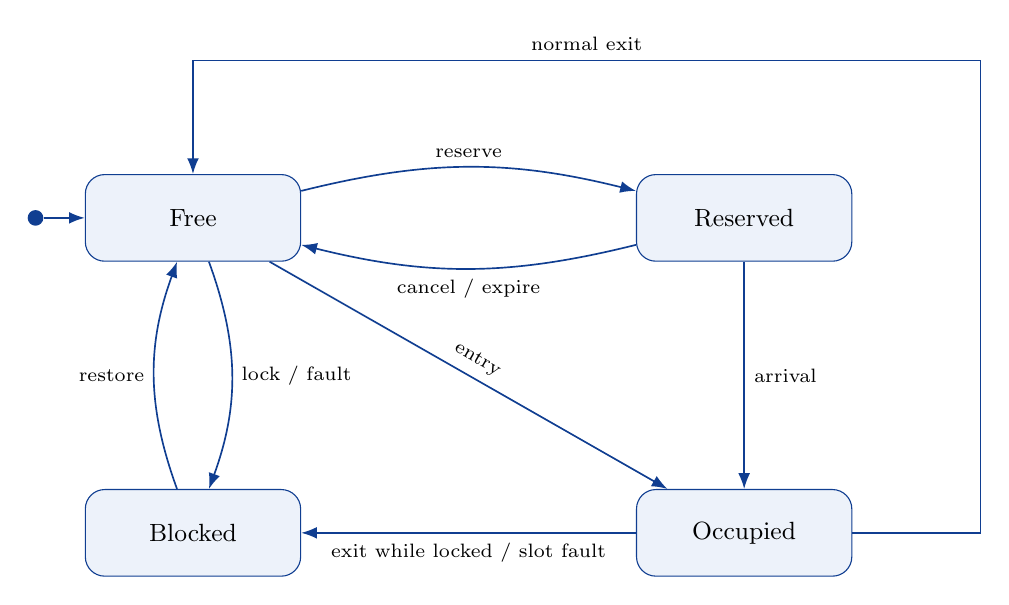
\begin{tikzpicture}
\node[state] (f) at (0,0) {Free};
\node[state] (r) at (7,0) {Reserved};
\node[state] (o) at (7,-4) {Occupied};
\node[state] (b) at (0,-4) {Blocked};
\node[circle,fill=navy,inner sep=2pt] (start) at (-2,0) {};
\draw[arr] (start)--(f);
\draw[arr] (f) to[bend left=14] node[above,font=\scriptsize]{reserve}(r);
\draw[arr] (r) to[bend left=14] node[below,font=\scriptsize]{cancel / expire}(f);
\draw[arr] (r)--node[right,font=\scriptsize]{arrival}(o);
\draw[arr] (f)--node[above,sloped,font=\scriptsize]{entry}(o);
\draw[arr] (o)--node[below,font=\scriptsize]{exit while locked / slot fault}(b);
\draw[arr] (b) to[bend left=20] node[left,font=\scriptsize]{restore}(f);
\draw[arr] (f) to[bend left=20] node[right,font=\scriptsize]{lock / fault}(b);
\draw[arr] (o.east)--(10,-4)--(10,2)--node[above,font=\scriptsize]{normal exit}(0,2)--(f.north);
\end{tikzpicture}}{Slot state machine; labels show representative events}{fig:slot-state}

\smallfigure{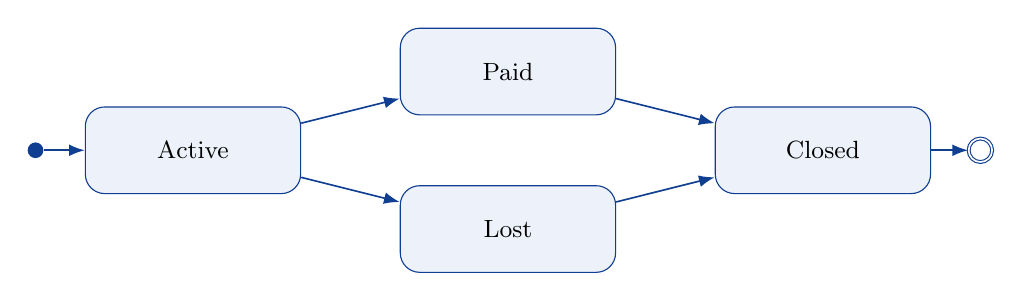
\begin{tikzpicture}
\node[state] (a) at (0,0) {Active};\node[state] (p) at (4,1) {Paid};\node[state] (l) at (4,-1) {Lost};\node[state] (c) at (8,0) {Closed};
\node[circle,fill=navy,inner sep=2pt] (i) at (-2,0) {};\node[circle,draw=navy,double,inner sep=3pt] (e) at (10,0) {};
\draw[arr] (i)--(a);\draw[arr] (a)--(p);\draw[arr] (a)--(l);\draw[arr] (p)--(c);\draw[arr] (l)--(c);\draw[arr] (c)--(e);
\end{tikzpicture}}{Ticket state machine}{fig:ticket-state}

\smallfigure{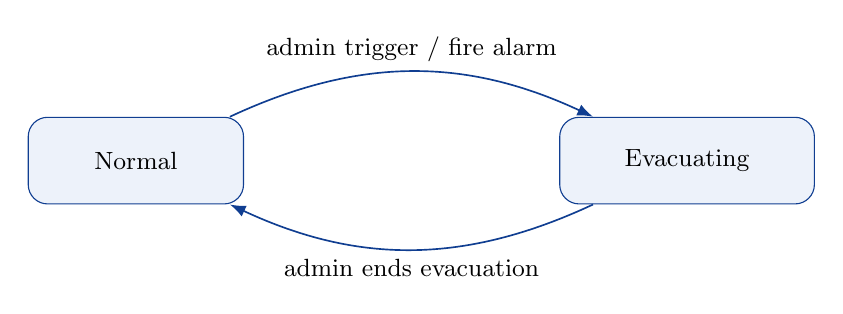
\begin{tikzpicture}
\node[state] (n) at (0,0) {Normal};\node[state,text width=30mm] (e) at (7,0) {Evacuating};
\draw[arr] (n) to[bend left=25] node[above,font=\small]{admin trigger / fire alarm}(e);
\draw[arr] (e) to[bend left=25] node[below,font=\small]{admin ends evacuation}(n);
\end{tikzpicture}}{Lot state machine}{fig:lot-state}

Locking a zone immediately moves only Free slots to Blocked. Occupied slots retain their vehicles and become Blocked on exit if the lock remains. Existing reservations are retained under UC-05. Evacuation cancels reservations before locking the lot. A sensor fault can change an Occupied slot to Blocked while its ticket remains, so invariants must consider fault flags and ticket links together.

\subsection{Ticket and Lot States}
An ordinary ticket moves from Active to Paid and then Closed; a lost ticket passes through Lost before Closed. A Closed ticket cannot return to Active. The lot has Normal and Evacuating modes. Only an administrator may end evacuation; a fire alarm may start it without an account. The diagrams represent software transitions and do not establish physical equipment interlocks.

\subsection{Hierarchy and Invariants}
\widefigure{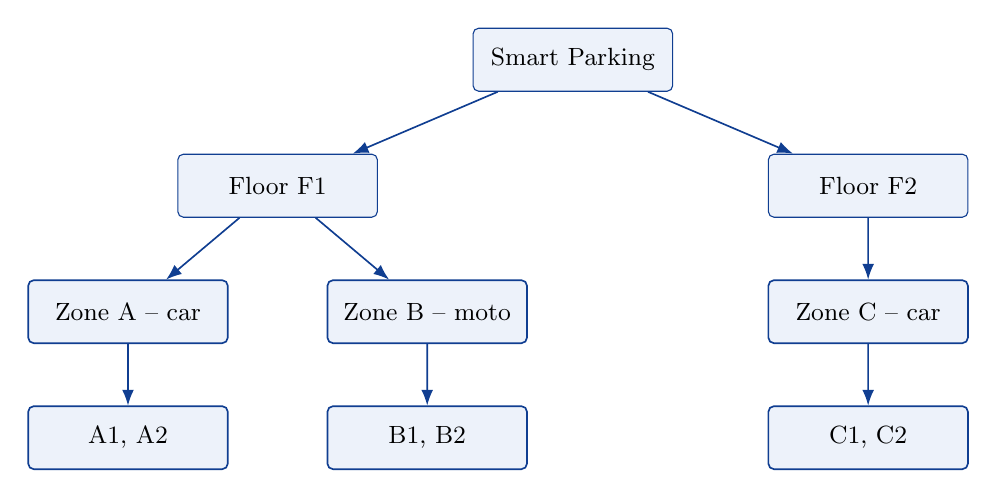
\begin{tikzpicture}[level distance=16mm,level 1/.style={sibling distance=75mm},level 2/.style={sibling distance=38mm},every node/.style={box,text width=23mm,minimum height=8mm,font=\small},edge from parent/.style={arr}]
\node {Smart Parking}
child {node {Floor F1} child {node {Zone A -- car} child {node {A1, A2}}} child {node {Zone B -- moto} child {node {B1, B2}}}}
child {node {Floor F2} child {node {Zone C -- car} child {node {C1, C2}}}};
\end{tikzpicture}}{Standard lot hierarchy: six slots on two floors}{fig:tree}

Relevant invariants include: each active ticket has a plate and valid slot; a slot is not assigned to two vehicles in sequential execution; availability equals the number of Free leaves; and no new ticket is issued during evacuation. Multiple threads or gates require atomic transactions and data locking. Transition checks in a single-process simulation do not establish protection against concurrent allocation races.

\section{Data Flow Diagram (DFD)}
\widefigure{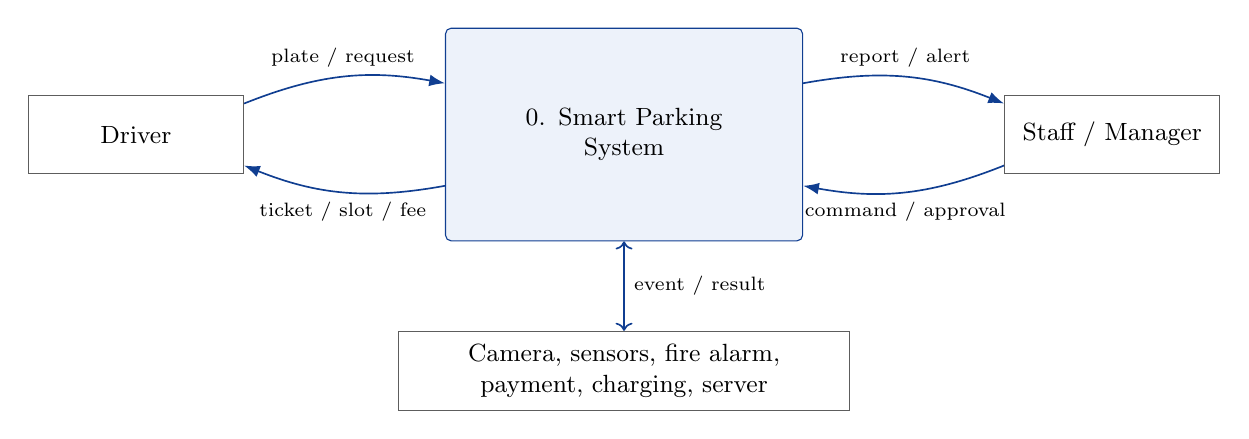
\begin{tikzpicture}
\node[box,text width=43mm,minimum height=27mm] (sps) at (0,0) {0. Smart Parking\\System};
\node[ext] (driver) at (-6.2,0) {Driver};
\node[ext] (staff) at (6.2,0) {Staff / Manager};
\node[ext,text width=55mm] (dev) at (0,-3) {Camera, sensors, fire alarm, payment, charging, server};
\draw[arr] (driver) to[bend left=16] node[above,font=\scriptsize]{plate / request}(sps);
\draw[arr] (sps) to[bend left=16] node[below,font=\scriptsize]{ticket / slot / fee}(driver);
\draw[arr] (staff) to[bend left=16] node[below,font=\scriptsize]{command / approval}(sps);
\draw[arr] (sps) to[bend left=16] node[above,font=\scriptsize]{report / alert}(staff);
\draw[arr,<->] (sps)--node[right,font=\scriptsize]{event / result}(dev);
\end{tikzpicture}}{Context-level DFD}{fig:dfd-context}

\widefigure{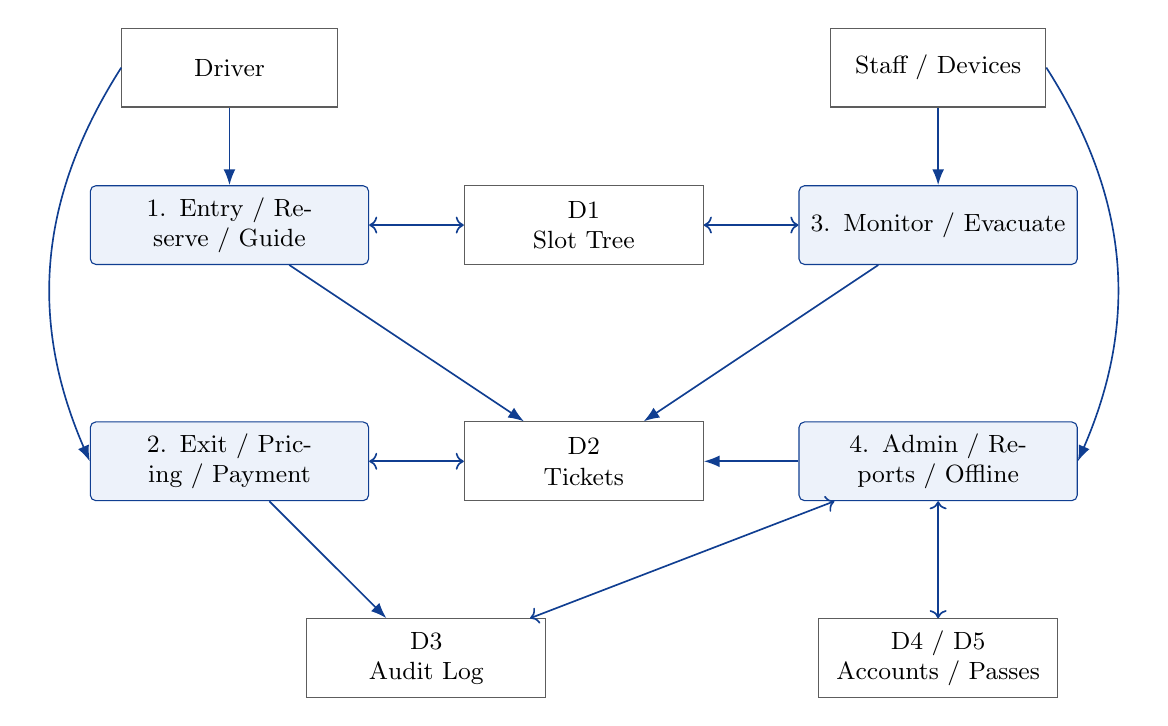
\begin{tikzpicture}
\node[ext] (driver) at (-1.5,4) {Driver};\node[ext] (staff) at (7.5,4) {Staff / Devices};
\node[box] (p1) at (-1.5,2) {1. Entry / Reserve / Guide};
\node[box] (p2) at (-1.5,-1) {2. Exit / Pricing / Payment};
\node[box] (p3) at (7.5,2) {3. Monitor / Evacuate};
\node[box] (p4) at (7.5,-1) {4. Admin / Reports / Offline};
\node[ext,text width=28mm] (d1) at (3,2) {D1\\Slot Tree};
\node[ext,text width=28mm] (d2) at (3,-1) {D2\\Tickets};
\node[ext,text width=28mm] (d3) at (1,-3.5) {D3\\Audit Log};
\node[ext,text width=28mm] (d4) at (7.5,-3.5) {D4 / D5\\Accounts / Passes};
\draw[arr] (driver)--(p1);\draw[arr] (driver.west) to[bend right=28] (p2.west);\draw[arr] (staff)--(p3);\draw[arr] (staff.east) to[bend left=28] (p4.east);
\draw[arr,<->] (p1)--(d1);\draw[arr,<->] (p3)--(d1);\draw[arr,<->] (p2)--(d2);\draw[arr] (p1)--(d2);\draw[arr] (p3)--(d2);\draw[arr] (p4)--(d2);
\draw[arr] (p2)--(d3);\draw[arr,<->] (p4)--(d3);\draw[arr,<->] (p4)--(d4);
\end{tikzpicture}}{Decomposed DFD with grouped processes}{fig:dfd-level1}

At context level, inputs are driver requests, staff commands, and device events; outputs are tickets, guidance, notifications, fees, and reports. The decomposed DFD groups processes into entry/reservations, exit/pricing, monitoring/safety, and administration/synchronization. Logical stores contain the slot tree, tickets, audit records, accounts, and monthly/VIP passes. These are logical stores implemented through memory and JSON, rather than five separately deployed databases.

Pricing reads tickets and pricing policies, records payment, and returns a result to the gate. Monitoring reconciles sensors against tickets and does not automatically delete a ticket on mismatch. Offline operation marks local records and clears marks on reconnection. The code has no actual transport protocol or multi-replica conflict resolution. A detailed Mermaid model with 19 processes is supplied in \texttt{data/diagrams.mmd} for comparison with the grouped DFD.

\section{Chapter Conclusion}
State machines define legal transitions; the hierarchy supports aggregation and allocation; DFDs show information sources and use. The three views complement one another but require additional failure-path and concurrency verification as the system grows.

Each view answers a different question. The state machines for slot, ticket, and lot decide which moves are allowed, and the code rejects any other move with an error. The Lot, Floor, Zone, and Slot tree decides how availability is counted, how a zone is locked, and how the nearest slot is found. The context and decomposed DFDs show where plate, payment, sensor, and alarm data enter and leave the system. Together they give the reviewer a way to check a requirement against structure, behavior, and data flow. Concurrent allocation remains untested, and the diagrams do not prove it.

\chapter{Non-functional Requirements \& Verification}
\section{ISO/IEC 25010 Classification}
The course template references ISO/IEC 25010:2011 and its eight product-quality characteristics~\cite{iso25010}. This report retains that edition as the comparison baseline. ISO/IEC 25010:2023 defines a nine-characteristic model~\cite{iso2023}; the terminology of the two editions should not be combined without review.
\begin{table}[H]\centering\small\caption{NFR mapping and interpretation by standard edition}
\begin{tabularx}{\linewidth}{L{18mm}L{46mm}X}\toprule
\textbf{ID} & \textbf{2011 reference category} & \textbf{Interpretation in this report}\\\midrule
NFR-01 & Performance efficiency & Slot-assignment response time.\\
NFR-02 & Reliability / availability & Gate-service availability.\\
NFR-03 & Usability & New attendants' ability to complete a task.\\
NFR-04 & Security / confidentiality & Protection of identifying and payment data.\\
NFR-05 & Performance efficiency / capacity & Growth in scale; quantitative workload targets are needed.\\
NFR-06 & System-level safety requirement & Safety is not treated as one of the eight product-quality characteristics of the 2011 edition.\\\bottomrule
\end{tabularx}\end{table}
The code in \texttt{rm.py} prints Safety directly for NFR-06. The dataset snapshot \url{data/dataset.json} retains the source category, while this report distinguishes its interpretation to avoid attributing it incorrectly to the 2011 product model. Adopting the 2023 baseline requires reviewing the entire mapping rather than merely changing the year in a heading.

\needspace{16\baselineskip}\section{Simulation Verification Results}
\subsection{Measurement Design and Environment}
\par\needspace{10\baselineskip}\begingroup\footnotesize\setlength{\tabcolsep}{4pt}
\begin{longtable}{>{\raggedright\arraybackslash}p{\dimexpr 0.22000\linewidth-2\tabcolsep\relax}>{\raggedright\arraybackslash}p{\dimexpr 0.78000\linewidth-2\tabcolsep\relax}}
\caption{Verification environment}\\
\toprule
\textbf{Property} & \textbf{Value} \\ \midrule
\endfirsthead
\multicolumn{2}{l}{\small\itshape Verification environment (continued)}\\
\toprule
\textbf{Property} & \textbf{Value} \\ \midrule
\endhead
\midrule
\multicolumn{2}{r}{\scriptsize Continued on the next page}\\
\endfoot
\bottomrule\endlastfoot
Recorded at & 2026-10-20T00:24:53.968899+07:00 \\
Python & 3.14.6 \\
Operating system & Windows-11-10.0.26200-SP0 \\
Processor & Intel64 Family 6 Model 183 Stepping 1, GenuineIntel \\
Execution & Sequential; single process; time.perf\_counter \\
\end{longtable}\endgroup

NFR-01 is measured using 1,000 sequential entry calls on a 1,000-car-slot lot in one process. Each call includes slot search, ticket creation, and in-memory logging. The 95th percentile is the 950th value in the sorted timing sequence. NFR-06 measures evacuation with 500 parked vehicles in a 1,000-slot lot. Neither measurement includes cameras, networking, payment, controllers, or mechanical barrier movement.

NFR-02 uses a 30-day model with random seed 2026, an outage probability of 0.4\% per hour, and outages lasting 5--20 minutes. This is assumption-based analysis, not operational uptime monitoring. Results depend on the assumptions and do not represent measured production reliability.
\par\needspace{11\baselineskip}\begingroup\footnotesize\setlength{\tabcolsep}{4pt}
\begin{longtable}{>{\raggedright\arraybackslash}p{\dimexpr 0.13000\linewidth-2\tabcolsep\relax}>{\raggedright\arraybackslash}p{\dimexpr 0.62000\linewidth-2\tabcolsep\relax}>{\raggedright\arraybackslash}p{\dimexpr 0.25000\linewidth-2\tabcolsep\relax}}
\caption{NFR results and evidence scope}\label{tab:nfr-results}\\
\toprule
\textbf{ID} & \textbf{Recorded result} & \textbf{Evidence type} \\ \midrule
\endfirsthead
\multicolumn{3}{l}{\small\itshape NFR results and evidence scope (continued)}\\
\toprule
\textbf{ID} & \textbf{Recorded result} & \textbf{Evidence type} \\ \midrule
\endhead
\midrule
\multicolumn{3}{r}{\scriptsize Continued on the next page}\\
\endfoot
\bottomrule\endlastfoot
NFR-01 & PASS (simulated): p95 = 0.928 ms over 1000 requests (target \textless{}= 1 second) & Sequential Python timing \\
NFR-02 & PASS (simulated): 99.98\% uptime, 7 min down in 30 days (target \textgreater{}= 99.5\%; modeled outages) & Assumed outage model \\
NFR-03 & Not evaluated with new users. & Not verified \\
NFR-04 & Storage and transport encryption are not implemented. & Not verified \\
NFR-05 & Metric/target missing; no acceptance conclusion. & Not verified \\
NFR-06 & PASS (simulated): barriers open in 0.346 ms with 500 cars parked (target \textless{}= 5 seconds) & Sequential Python timing \\
\end{longtable}\endgroup

The timings in Table~\ref{tab:nfr-results} come from a dedicated measurement run. TC-04 and the evacuation test in Table~\ref{tab:tests} measure the same quantities in a separate run, so the numbers differ slightly; both vary with the machine and only the comparison with the target matters.

\subsection{Requirements Not Fully Verified}
NFR-03 has not been tested with new staff; lost-ticket task time should be measured after 20 minutes of training. NFR-04 has no encryption evidence. NFR-05 lacks a threshold. A proposed extension is to define 1,000 slots, gate count, and concurrent workload before measuring p95 and consistency. This proposal is not approved in the workbook.

\section{Chapter Conclusion}
Three NFRs have results from simulation timing or assumption-based analysis, which do not establish an end-to-end SLA. Usability, encryption, and scalability require further evidence.

The measured results are the slot-assignment p95 time (NFR-01, target one second), the barrier-opening time during evacuation (NFR-06, target five seconds), and the uptime from an assumed outage model (NFR-02, target 99.5\%). The two timings are far below their targets, but they come from sequential Python calls on one machine, so they show that the logic is cheap, not that a real site meets the target. NFR-03 has no test with new staff, NFR-04 has no encryption, and NFR-05 has no threshold, so none of the three can be accepted yet. The report therefore separates what was measured, what was modeled, and what remains open.

\chapter{Validation, Verification \& Change Management}
\section{Requirements Traceability Matrix}
\par\needspace{8\baselineskip}\begingroup\scriptsize\setlength{\tabcolsep}{4pt}
\begin{longtable}{>{\raggedright\arraybackslash}p{\dimexpr 0.60000\linewidth-2\tabcolsep\relax}>{\raggedright\arraybackslash}p{\dimexpr 0.20000\linewidth-2\tabcolsep\relax}>{\raggedright\arraybackslash}p{\dimexpr 0.20000\linewidth-2\tabcolsep\relax}}
\caption{Functional requirement link coverage}\label{tab:coverage}\\
\toprule
\textbf{Criterion} & \textbf{Count} & \textbf{Coverage} \\ \midrule
\endfirsthead
\multicolumn{3}{l}{\small\itshape Functional requirement link coverage (continued)}\\
\toprule
\textbf{Criterion} & \textbf{Count} & \textbf{Coverage} \\ \midrule
\endhead
\midrule
\multicolumn{3}{r}{\scriptsize Continued on the next page}\\
\endfoot
\bottomrule\endlastfoot
Has a use-case link & 31 & 100\% \\
Has a test-case link & 31 & 100\% \\
Has a direct elicitation-session link & 21 & 68\% \\
\end{longtable}\endgroup

\par\begingroup\scriptsize\setlength{\tabcolsep}{4pt}
\begin{longtable}{>{\raggedright\arraybackslash}p{\dimexpr 0.13000\linewidth-2\tabcolsep\relax}>{\raggedright\arraybackslash}p{\dimexpr 0.27000\linewidth-2\tabcolsep\relax}>{\raggedright\arraybackslash}p{\dimexpr 0.34000\linewidth-2\tabcolsep\relax}>{\raggedright\arraybackslash}p{\dimexpr 0.26000\linewidth-2\tabcolsep\relax}}
\caption{Functional and non-functional traceability}\label{tab:trace}\\
\toprule
\textbf{Requirement} & \textbf{Use case} & \textbf{Test case} & \textbf{HZ / CR / EL} \\ \midrule
\endfirsthead
\multicolumn{4}{l}{\small\itshape Functional and non-functional traceability (continued)}\\
\toprule
\textbf{Requirement} & \textbf{Use case} & \textbf{Test case} & \textbf{HZ / CR / EL} \\ \midrule
\endhead
\midrule
\multicolumn{4}{r}{\scriptsize Continued on the next page}\\
\endfoot
\bottomrule\endlastfoot
REQ-01 & UC-01, UC-07 & TC-01, TC-02, TC-04 & HZ-03; CR-02; EL-01 \\
REQ-02 & UC-01, UC-15 & TC-41, TC-46 & CR-02; EL-01 \\
REQ-03 & UC-02, UC-17 & TC-03, TC-07, TC-26 & HZ-02; CR-01; EL-01 \\
REQ-04 & UC-02 & TC-25 & EL-01 \\
REQ-05 & UC-03, UC-13 & TC-05, TC-27, TC-28 & CR-02; EL-03 \\
REQ-06 & UC-04 & TC-06, TC-29 & EL-03 \\
REQ-07 & UC-06 & TC-10, TC-31, TC-32 & EL-01 \\
REQ-08 & UC-05 & TC-09, TC-15, TC-30, TC-46 & EL-02 \\
REQ-09 & UC-05, UC-10, UC-12, UC-14, UC-16, UC-17, UC-19 & TC-08, TC-20, TC-40, TC-51, TC-55, TC-56 & HZ-05; EL-02 \\
REQ-10 & UC-16 & TC-43 & EL-02 \\
REQ-11 & UC-07, UC-21 & TC-11, TC-12, TC-13 & HZ-06; EL-04 \\
REQ-12 & UC-08, UC-18 & TC-14, TC-15 & EL-05 \\
REQ-13 & UC-09 & TC-16, TC-17 & HZ-08; EL-04 \\
REQ-14 & UC-09 & TC-18 & EL-04 \\
REQ-15 & UC-10, UC-22 & TC-19, TC-20, TC-21, TC-22, TC-44, TC-45, TC-66 & HZ-07; EL-04 \\
REQ-16 & UC-11 & TC-07, TC-23 & HZ-09; CR-01; EL-05 \\
REQ-17 & UC-11 & TC-24 & HZ-09; CR-01; EL-05 \\
REQ-18 & UC-05, UC-12 & TC-33, TC-34, TC-35 & HZ-05; EL-02 \\
REQ-19 & UC-13 & TC-36, TC-37 & EL-03 \\
REQ-20 & UC-14 & TC-38, TC-39, TC-40 & EL-05 \\
REQ-21 & UC-16 & TC-42, TC-47 & EL-05 \\
REQ-22 & UC-17 & TC-50, TC-51 & HZ-02, HZ-12 \\
REQ-23 & UC-18, UC-19 & TC-52, TC-53, TC-54, TC-55, TC-56 & --- \\
REQ-24 & UC-20 & TC-57 & CR-02 \\
REQ-25 & UC-20 & TC-58, TC-59 & CR-02 \\
REQ-26 & UC-02, UC-21 & TC-60, TC-61, TC-62 & HZ-10 \\
REQ-27 & UC-11 & TC-48 & --- \\
REQ-28 & UC-11 & TC-49 & HZ-09 \\
REQ-29 & UC-19, UC-22 & TC-56, TC-63, TC-64, TC-66 & HZ-11 \\
REQ-30 & UC-22 & TC-65 & HZ-11 \\
REQ-31 & UC-01, UC-02 & TC-67 & HZ-04 \\
NFR-01 & --- & TC-04 & EL-02 \\
NFR-02 & --- & TC-67 & HZ-04, HZ-11; EL-02 \\
NFR-03 & --- & --- & --- \\
NFR-04 & --- & --- & HZ-01 \\
NFR-05 & --- & --- & --- \\
NFR-06 & --- & TC-22 & HZ-07; EL-04 \\
\end{longtable}\endgroup

Here, 100\% coverage means that each functional requirement has at least one use-case link and one test-case link. It does not mean every clause is tested, every branch is executed, or stakeholders have approved the requirement. REQ-07, in particular, still lacks acceptance criteria despite having simulation tests.

Dependencies form a directed graph, and a requirement may have multiple parents. The tool displays that graph as a tree, so an identifier can appear more than once. Impact analysis uses sets to avoid duplicate counting. The current dataset version has no general-purpose dependency-cycle validation.

\section{Automated Test Results}
\subsection{Scope and Method}
The runner maps TC-01 through TC-67 to functions in \texttt{checks.py}. Each function operates on separate simulation objects and checks outcomes with assertions. The report calls \texttt{checks.run\_tests(data)} directly rather than invoking workbook write-back. The original data is preserved, and the resulting execution snapshot is stored under \texttt{evidence/}.
\par\needspace{6\baselineskip}\begingroup\footnotesize\setlength{\tabcolsep}{4pt}
\begin{longtable}{>{\raggedright\arraybackslash}p{\dimexpr 0.25000\linewidth-2\tabcolsep\relax}>{\raggedright\arraybackslash}p{\dimexpr 0.25000\linewidth-2\tabcolsep\relax}>{\raggedright\arraybackslash}p{\dimexpr 0.25000\linewidth-2\tabcolsep\relax}>{\raggedright\arraybackslash}p{\dimexpr 0.25000\linewidth-2\tabcolsep\relax}}
\caption{Recorded automated test summary}\\
\toprule
\textbf{Total} & \textbf{Passed} & \textbf{Failed} & \textbf{Not Run} \\ \midrule
\endfirsthead
\multicolumn{4}{l}{\small\itshape Recorded automated test summary (continued)}\\
\toprule
\textbf{Total} & \textbf{Passed} & \textbf{Failed} & \textbf{Not Run} \\ \midrule
\endhead
\midrule
\multicolumn{4}{r}{\scriptsize Continued on the next page}\\
\endfoot
\bottomrule\endlastfoot
67 & 67 & 0 & 0 \\
\end{longtable}\endgroup

The tests cover normal operation, capacity shortages, authorization, fee boundaries, camera failures, sensors, evacuation, monthly/VIP passes, EVs, exit-plate verification, and offline behavior. Important boundaries include the 15/16-minute grace period, 24/25-hour cap, 79/80\% recognition confidence, and the failed-login count that triggers lockout.
Table~\ref{tab:tests} lists every test with its recorded result. NFR-01 and NFR-06 timings quoted there come from the test run and differ slightly from Table~\ref{tab:nfr-results}, which comes from a separate measurement run; both vary with the machine.
\par\begingroup\scriptsize\setlength{\tabcolsep}{4pt}
\begin{longtable}{>{\raggedright\arraybackslash}p{\dimexpr 0.23000\linewidth-2\tabcolsep\relax}>{\raggedright\arraybackslash}p{\dimexpr 0.28000\linewidth-2\tabcolsep\relax}>{\raggedright\arraybackslash}p{\dimexpr 0.49000\linewidth-2\tabcolsep\relax}}
\caption{Complete results of 67 automated tests}\label{tab:tests}\\
\toprule
\textbf{ID / requirements} & \textbf{Test objective} & \textbf{Actual result} \\ \midrule
\endfirsthead
\multicolumn{3}{l}{\small\itshape Complete results of 67 automated tests (continued)}\\
\toprule
\textbf{ID / requirements} & \textbf{Test objective} & \textbf{Actual result} \\ \midrule
\endhead
\midrule
\multicolumn{3}{r}{\scriptsize Continued on the next page}\\
\endfoot
\bottomrule\endlastfoot
TC-01 / REQ-01 & Entry assigns the nearest free slot of the matching type & Passed: Ticket issued; slot A1 assigned. \\
TC-02 / REQ-01 & Entry is rejected when the zone is full & Passed: Entry rejected ('zone full'); rejection logged. \\
TC-03 / REQ-03 & Fee is calculated correctly for a 2h30 stay & Passed: Fee = 30000 VND. \\
TC-04 / REQ-01; NFR-01 & Slot assignment responds within 1 second under normal load & Passed: p95 = 2.332 ms over 1000 requests. \\
TC-05 / REQ-05 & Reserved slot is not given to another vehicle & Passed: Other car got A2; VIP-1 got A1. \\
TC-06 / REQ-06 & Vehicle is located by plate number & Passed: Found: Smart Parking \textgreater{} F1 \textgreater{} A \textgreater{} A2. \\
TC-07 / REQ-03; REQ-16 & Peak-hour rate is applied once CR-01 is implemented & Passed: CR-01 implemented: 17:00-18:00 charged 15000 VND (1.5 x 10000). \\
TC-08 / REQ-09 & Attendant account cannot lock a zone & Passed: PermissionError raised; denial logged. \\
TC-09 / REQ-08 & Locked zone is not assigned to new vehicles & Passed: Car assigned C1 (zone A blocked). \\
TC-10 / REQ-07 & Lost ticket is charged the maximum daily fee plus penalty & Passed: Charged 290000 VND (24h x 10000 + 50000). \\
TC-11 / REQ-11 & Plate with high confidence is accepted automatically & Passed: Plate 29A-111 accepted at 95\% confidence. \\
TC-12 / REQ-11 & Plate with low confidence requires manual entry & Passed: 55\% confidence: manual entry requested and accepted. \\
TC-13 / REQ-11 & Camera offline falls back to manual entry & Passed: Manual entry required; camera\_offline logged. \\
TC-14 / REQ-12 & Nearest free slot is assigned & Passed: Assigned B1 (10 m), not A1 (40 m). \\
TC-15 / REQ-12; REQ-08 & Next nearest slot is assigned when the nearest zone is locked & Passed: Zone B locked: assigned A1. \\
TC-16 / REQ-13 & Sensor mismatch raises alerts & Passed: Alerts: missing\_vehicle, unauthorized\_vehicle. \\
TC-17 / REQ-13 & Silent sensor blocks its slot & Passed: B2 blocked on silence, freed on recovery. \\
TC-18 / REQ-14 & Overstay alert after 24 hours & Passed: 29A-111 parked 25 h in A1 (limit 24 h) \\
TC-19 / REQ-15 & Evacuation opens barriers and stops new entries & Passed: Barriers open; entry rejected; exit charged 0 VND. \\
TC-20 / REQ-15; REQ-09 & Attendant cannot trigger evacuation & Passed: PermissionError raised; denial logged. \\
TC-21 / REQ-15 & Fire alarm starts evacuation without login & Passed: Evacuation started by fire alarm; barriers open. \\
TC-22 / REQ-15; NFR-06 & Barriers open within 5 seconds of the evacuation trigger & Passed: Barriers open in 0.404 ms (500 cars parked). \\
TC-23 / REQ-16 & Peak-hour multiplier applies only to peak hours & Passed: Fee = 25000 VND (10000 + 15000). \\
TC-24 / REQ-17 & Occupancy surcharge applies above 80\% occupancy & Passed: 3rd car base fee; 4th car (100\% occupancy) 12500 VND = 125\% of 10000. \\
TC-25 / REQ-04 & Barrier opens only after payment is made & Passed: Failed payment: slot stays occupied; after payment the slot is free. \\
TC-26 / REQ-03 & Exit with an unknown ticket is refused & Passed: Exit refused: ticket not found. \\
TC-27 / REQ-05 & Reservation is rejected when no slot is free & Passed: 5th reservation rejected (4 car slots reserved). \\
TC-28 / REQ-05 & No-show reservation is released after 15 minutes & Passed: A1 released at 10:46. \\
TC-29 / REQ-06 & Locate rejects an unknown plate & Passed: Plate NOPE: vehicle not found. \\
TC-30 / REQ-08 & Occupied slot stays occupied when its zone is locked & Passed: A1 occupied after lock; blocked after exit. \\
TC-31 / REQ-07 & Lost ticket without an entry record is escalated & Passed: no entry record: escalate to the Parking Manager. \\
TC-32 / REQ-07 & Lost ticket without proof of ownership is refused & Passed: Exit refused; refusal logged. \\
TC-33 / REQ-18 & Valid login returns the account role & Passed: admin1 logged in with role admin. \\
TC-34 / REQ-18 & Wrong password is rejected & Passed: Login rejected; failed attempts: 1. \\
TC-35 / REQ-18 & Account is locked after 3 failed attempts & Passed: account locked (correct password refused after 3 failures). \\
TC-36 / REQ-19 & Cancelling a reservation frees the slot & Passed: A1 released and assigned to the next car. \\
TC-37 / REQ-19 & Cancelling a missing reservation is reported & Passed: Cancel NOPE: reservation not found. \\
TC-38 / REQ-20 & Rate change applies to new tickets only & Passed: Car A pays 10000; car B pays 12000. \\
TC-39 / REQ-20 & Zone added at runtime is assignable at once & Passed: Zone D added; the next car got D1. \\
TC-40 / REQ-20; REQ-09 & Attendant cannot change rates or add zones & Passed: Both attempts denied. \\
TC-41 / REQ-02 & Availability counts match the slot states & Passed: A 0/2, F1 2/4, lot 4/6 free. \\
TC-42 / REQ-21 & Revenue per zone and floor sums to the total & Passed: Zones \{'A': 20000, 'C': 10000\} = floors \{'F1': 20000, 'F2': 10000\} = total 30000. \\
TC-43 / REQ-10 & Audit log records entry, payment and exit & Passed: Audit events: entry, payment, exit. \\
TC-44 / REQ-15 & Ending an evacuation restores normal operation & Passed: Barriers closed, slots unblocked, new entry accepted. \\
TC-45 / REQ-15 & Evacuation cancels reservations & Passed: Reservation cancelled; A1 blocked. \\
TC-46 / REQ-02; REQ-08 & Locked zone shows zero free slots & Passed: Zone A shows 0 free slots. \\
TC-47 / REQ-21 & Report for a period without payments shows zero & Passed: Revenue 0, 0 payments. \\
TC-48 / REQ-27 & A stay of 15 minutes is free & Passed: 15 min = 0 VND; 16 min = 10000 VND. \\
TC-49 / REQ-28 & The fee of a started 24 hours is capped & Passed: 24 h = 100000 VND (cap); 25 h = 110000 VND. \\
TC-50 / REQ-22 & An approved fee override replaces the calculated fee & Passed: ticket fee 5000 VND (was 20000); exit charged 5000; logged: override\_requested, override\_approved \\
TC-51 / REQ-22; REQ-09 & Invalid, unapproved or rejected overrides do not change the fee & Passed: rejected: override needs a non-negative amount and a reason; manager rejects OV-1: fee stays 20000 VND; attendant approval denied: manager or admin only \\
TC-52 / REQ-23 & A monthly pass parks free of charge & Passed: Monthly pass: 5 h stay costs 0 VND. \\
TC-53 / REQ-23 & Only VIP pass holders get VIP slots & Passed: VIP holder: V1; monthly holder: A1; ordinary car: A2. \\
TC-54 / REQ-23 & An expired pass pays the normal fee & Passed: Expired pass: expiry logged, fee 20000 VND. \\
TC-55 / REQ-23; REQ-09 & Administrator registers and removes a pass & Passed: pass stored; logged: pass\_added (monthly until 2026-11-16); MON-1 removed; removal logged \\
TC-56 / REQ-23; REQ-09; REQ-29 & Invalid, unauthorized or offline pass registration is refused & Passed: rejected: invalid pass (kind monthly|vip, end date in the future); invalid pass (kind monthly|vip, end date in the future); attendant denied: administrator only; refused: pass registration needs the central server (offline mode) \\
TC-57 / REQ-24 & EVs get EV slots and cars never do & Passed: EVs got E1 and E2; third EV rejected; the car got A1. \\
TC-58 / REQ-25 & The energy price is added to the fee & Passed: Fee 59000 VND (24000 parking + 35000 energy). \\
TC-59 / REQ-25 & A bad energy reading is rejected & Passed: 0 kWh and a car reading were rejected. \\
TC-60 / REQ-26 & A matching exit plate lets the vehicle leave & Passed: Matching plate: vehicle left. \\
TC-61 / REQ-26 & A plate mismatch keeps the barrier closed & Passed: Mismatch: exit refused, slot still occupied, mismatch logged. \\
TC-62 / REQ-26 & An attendant can approve a mismatch or an unreadable plate & Passed: attendant approves: vehicle leaves (10000 VND), approval logged; unreadable plate: barrier stays closed; a guest cannot approve \\
TC-63 / REQ-29 & Gates keep working offline & Passed: Offline: entry and cash exit worked; 3 records marked. \\
TC-64 / REQ-29 & Online payment and reservations are refused offline & Passed: online refused: payment gateway unavailable: pay cash or card at the booth; slot Occupied; refused offline: reservation needs the central server (offline mode); pass registration needs the central server (offline mode) \\
TC-65 / REQ-30 & Records are synchronized when the network returns & Passed: 1 record synchronized; marks cleared; count logged. \\
TC-66 / REQ-29; REQ-15 & Evacuation works offline & Passed: evacuation offline: barriers OPEN, exit free of charge \\
TC-67 / REQ-31; NFR-02 & Barrier stays open while a vehicle is present or the sensor fails & Passed: Barrier stayed open with a vehicle present, a sensor fault, and power loss (3 refusals logged); closed when clear. \\
\end{longtable}\endgroup


\subsection{Requirements Data Quality Assessment}
\par\needspace{12\baselineskip}\begingroup\footnotesize\setlength{\tabcolsep}{4pt}
\begin{longtable}{>{\raggedright\arraybackslash}p{\dimexpr 0.12000\linewidth-2\tabcolsep\relax}>{\raggedright\arraybackslash}p{\dimexpr 0.16000\linewidth-2\tabcolsep\relax}>{\raggedright\arraybackslash}p{\dimexpr 0.72000\linewidth-2\tabcolsep\relax}}
\caption{Requirements data quality findings}\label{tab:quality}\\
\toprule
\textbf{Level} & \textbf{ID} & \textbf{Finding} \\ \midrule
\endfirsthead
\multicolumn{3}{l}{\small\itshape Requirements data quality findings (continued)}\\
\toprule
\textbf{Level} & \textbf{ID} & \textbf{Finding} \\ \midrule
\endhead
\midrule
\multicolumn{3}{r}{\scriptsize Continued on the next page}\\
\endfoot
\bottomrule\endlastfoot
ERROR & REQ-07 & missing acceptance criteria \\
ERROR & NFR-05 & not measurable: metric or target value missing \\
WARN & REQ-07 & not atomic: description joins several actions (split into separate requirements) \\
WARN & REQ-10 & not atomic: description joins several actions (split into separate requirements) \\
INFO & REQ-07 & Must requirement still Proposed (needs approval) \\
INFO & REQ-10 & Must requirement still Proposed (needs approval) \\
INFO & REQ-15 & Must requirement still Proposed (needs approval) \\
\end{longtable}\endgroup

The two ERROR findings concern specification and measurement data; they remain even when every test is Passed. Atomicity warnings use a comma-and-conjunction heuristic and require analyst review. INFO findings identify Must requirements that remain Proposed, so business approval is needed before establishing an official baseline.

Further specification/implementation gaps include the lost-ticket rule versus the daily cap, calls to \texttt{exit} without an observed plate, zone locks before and after evacuation, and persistence of dynamically added zones. Reporting these gaps does not change the project's source code.

\section{Requirements Change Management}
The proposed process records a CR, identifies directly affected requirements, calculates dependency closure, reviews use cases/tests/risks, estimates effort, obtains a decision, updates the baseline, and runs regression tests. The status \emph{Implemented} in the workbook means the change was applied in the simulation, not accepted on a real installation.
\par\needspace{7\baselineskip}\begingroup\footnotesize\setlength{\tabcolsep}{4pt}
\begin{longtable}{>{\raggedright\arraybackslash}p{\dimexpr 0.12000\linewidth-2\tabcolsep\relax}>{\raggedright\arraybackslash}p{\dimexpr 0.20000\linewidth-2\tabcolsep\relax}>{\raggedright\arraybackslash}p{\dimexpr 0.52000\linewidth-2\tabcolsep\relax}>{\raggedright\arraybackslash}p{\dimexpr 0.16000\linewidth-2\tabcolsep\relax}}
\caption{Impact summary for the two change requests}\label{tab:changes}\\
\toprule
\textbf{CR} & \textbf{Direct requirements} & \textbf{Impact closure (requirements, use cases, tests)} & \textbf{Sample estimate} \\ \midrule
\endfirsthead
\multicolumn{4}{l}{\small\itshape Impact summary for the two change requests (continued)}\\
\toprule
\textbf{CR} & \textbf{Direct requirements} & \textbf{Impact closure (requirements, use cases, tests)} & \textbf{Sample estimate} \\ \midrule
\endhead
\midrule
\multicolumn{4}{r}{\scriptsize Continued on the next page}\\
\endfoot
\bottomrule\endlastfoot
CR-01 / Implemented & REQ-03, REQ-16, REQ-17 & 16 requirements (REQ-03, REQ-04, REQ-07, REQ-10, REQ-16, REQ-17, REQ-20, REQ-21, REQ-22, REQ-23, REQ-25, REQ-26, REQ-27, REQ-28, REQ-29, REQ-30); 11 use cases; 33 tests & cost 5 days; schedule 7 days \\
CR-02 / Implemented & REQ-01, REQ-02, REQ-05, REQ-24, REQ-25 & 29 requirements (REQ-01, REQ-02, REQ-03, REQ-04, REQ-05, REQ-06, REQ-07, REQ-08, REQ-10, REQ-11, REQ-12, REQ-13, REQ-14, REQ-15, REQ-16, REQ-17, REQ-19, REQ-20, REQ-21, REQ-22, REQ-23, REQ-24, REQ-25, REQ-26, REQ-27, REQ-28, REQ-29, REQ-30, REQ-31); 21 use cases; 63 tests & cost 3 days; schedule 3 days \\
\end{longtable}\endgroup

CR-01 adds peak-hour and occupancy pricing. Regression should include grace periods, passes, and revenue recording because they share fee calculation. CR-02 adds EV allocation and charging and has broad impact through the original allocation dependency. The returned impact set is a conservative review aid; final regression priorities and scope still require business interpretation.

\section{Chapter Conclusion}
The recorded execution shows the existing suite passing on the simulation, while traceability identifies the scope of changes. Specification quality, approval, and behavioral coverage require separate assessment. A passing-test percentage cannot replace requirements validation.

The suite contains 67 automated tests and all 67 pass; every functional requirement links to at least one use case and one test (Table~\ref{tab:coverage}). The quality checker still reports two errors, two warnings, and three informational findings, which no test can remove, because they concern the wording of requirements and not the behavior of the code. The impact of the two change requests was computed through the dependency tree (Table~\ref{tab:changes}), and both are marked Implemented in the simulation. That status does not mean acceptance on a real installation. Validation by real stakeholders is the missing step.

\chapter{Safety-Critical Systems, RE Tooling \& Integration}
\section{Safety Risk Analysis}
Each hazard records a cause, consequence, severity S, and likelihood L. This report uses $R=S\times L$ to prioritize review within the sample dataset. S has four levels and L has three; the workbook does not quantify the meaning of each level, so scores support only internal case-study comparisons.
\par\needspace{9\baselineskip}\begingroup\footnotesize\setlength{\tabcolsep}{4pt}
\begin{longtable}{>{\raggedright\arraybackslash}p{\dimexpr 0.10000\linewidth-2\tabcolsep\relax}>{\raggedright\arraybackslash}p{\dimexpr 0.30000\linewidth-2\tabcolsep\relax}>{\raggedright\arraybackslash}p{\dimexpr 0.30000\linewidth-2\tabcolsep\relax}>{\raggedright\arraybackslash}p{\dimexpr 0.30000\linewidth-2\tabcolsep\relax}}
\caption{Risk matrix S x L}\label{tab:risk-grid}\\
\toprule
\textbf{S / L} & \textbf{1} & \textbf{2} & \textbf{3} \\ \midrule
\endfirsthead
\multicolumn{4}{l}{\small\itshape Risk matrix S x L (continued)}\\
\toprule
\textbf{S / L} & \textbf{1} & \textbf{2} & \textbf{3} \\ \midrule
\endhead
\midrule
\multicolumn{4}{r}{\scriptsize Continued on the next page}\\
\endfoot
\bottomrule\endlastfoot
4 & HZ-04, HZ-07 & HZ-01 & --- \\
3 & --- & HZ-05, HZ-10 & HZ-06, HZ-11 \\
2 & --- & HZ-09 & HZ-02, HZ-03, HZ-08, HZ-12 \\
1 & --- & --- & --- \\
\end{longtable}\endgroup

\par\begingroup\footnotesize\setlength{\tabcolsep}{4pt}
\begin{longtable}{>{\raggedright\arraybackslash}p{\dimexpr 0.22000\linewidth-2\tabcolsep\relax}>{\raggedright\arraybackslash}p{\dimexpr 0.10000\linewidth-2\tabcolsep\relax}>{\raggedright\arraybackslash}p{\dimexpr 0.08000\linewidth-2\tabcolsep\relax}>{\raggedright\arraybackslash}p{\dimexpr 0.38000\linewidth-2\tabcolsep\relax}>{\raggedright\arraybackslash}p{\dimexpr 0.22000\linewidth-2\tabcolsep\relax}}
\caption{Hazard register and mitigation scope (ordered by R)}\label{tab:hazards}\\
\toprule
\textbf{ID / hazard} & \textbf{S / L / R} & \textbf{SIL} & \textbf{Mitigation and limitations} & \textbf{Traceability} \\ \midrule
\endfirsthead
\multicolumn{5}{l}{\small\itshape Hazard register and mitigation scope (ordered by R) (continued)}\\
\toprule
\textbf{ID / hazard} & \textbf{S / L / R} & \textbf{SIL} & \textbf{Mitigation and limitations} & \textbf{Traceability} \\ \midrule
\endhead
\midrule
\multicolumn{5}{r}{\scriptsize Continued on the next page}\\
\endfoot
\bottomrule\endlastfoot
HZ-06 Plate misrecognition & 3 / 3 / 9 & SIL-1 & 80\% threshold; manual fallback; confidence is simulated. & REQ-11 \\
HZ-11 Network loss stops gates & 3 / 3 / 9 & SIL-1 & Local entry/exit, marked logs; actual network synchronization is absent. & REQ-29; REQ-30; NFR-02 \\
HZ-01 Owner data exposure & 4 / 2 / 8 & SIL-2 & Encrypt backups and restrict access; no encryption evidence. & NFR-04 \\
HZ-02 Incorrect fees & 2 / 3 / 6 & QM & Test time/time-zone boundaries; overrides need manager approval. & REQ-03; REQ-22 \\
HZ-03 Duplicate slot assignment & 2 / 3 / 6 & QM & Reject repeated Occupied transitions; concurrent races are unverified. & REQ-01 \\
HZ-05 Unauthorized zone changes & 3 / 2 / 6 & SIL-1 & Authenticate, lock after three failures, and restrict to admin. & REQ-18; REQ-09 \\
HZ-08 Missing/incorrect sensor data & 2 / 3 / 6 & QM & Reconcile with tickets, alert, and block faulty slots. & REQ-13 \\
HZ-10 Exit with another ticket & 3 / 2 / 6 & SIL-1 & Compare exit and ticket plates; approval and logging on mismatch. & REQ-26 \\
HZ-12 Override abuse & 2 / 3 / 6 & QM & Separate request/approval roles; enforce distinct user identities in future. & REQ-22 \\
HZ-04 Barrier strikes a vehicle & 4 / 1 / 4 & SIL-2 & The gate refuses to close on a vehicle, a sensor fault, or power loss (REQ-31); no physical interlock is tested. & NFR-02; REQ-31 \\
HZ-07 Evacuation barriers fail to open & 4 / 1 / 4 & SIL-2 & Fail-open and payment bypass; physical and power-loss tests are needed. & REQ-15; NFR-06 \\
HZ-09 Excessive dynamic fees & 2 / 2 / 4 & QM & Fixed multipliers 1.5 x 1.25; show breakdown; clarify the cap. & REQ-16; REQ-17; REQ-28 \\
\end{longtable}\endgroup

SIL-1, SIL-2, and QM labels are preserved for source traceability. The \texttt{sil\_rule} function derives a label from severity alone. This is an educational convention, and there is no analysis or evidence supporting a claim of certified safety integrity. PII exposure, fraud, and revenue discrepancies also appear in the hazard register despite differing from physical injury risks.

The simulated policy keeps a barrier open on sensor failure, vehicle presence, or power loss. Separately, evacuation bypasses payment and blocks new tickets. REQ-31 makes this explicit: \texttt{close\_gate} calls \texttt{close\_barrier} and refuses to close on a vehicle, a sensor fault, or power loss (TC-67). The logic is not connected to hardware, so no physical interlock is demonstrated; HZ-04 is therefore covered by a requirement and a software test only. HZ-01 encryption has no verification demonstration. Other hazards have logical demonstrations, but HZ-03 has not been tested under concurrent allocation.

REQ-22 separates roles: an attendant requests an override, and a manager or administrator approves it. The code checks roles, not identities, so one person holding both roles could request and approve an override. This limitation matters if the mechanism is used operationally.

\section{Integrated Requirements Management Tool}
\begin{table}[H]\centering\small\caption{Modules and responsibilities}
\begin{tabularx}{\linewidth}{L{28mm}X}\toprule
File & Responsibility\\\midrule
\texttt{parking.py} & Entry point, menus, interactive mode, and Markdown appendix export.\\
\texttt{rm.py} & Excel loading, quality checks, traceability, dependencies, CR impact, risk matrices, and Mermaid export.\\
\texttt{sim.py} & Lot hierarchy, tickets, states, pricing, authorization, sensors, evacuation, and persistence.\\
\texttt{checks.py} & 22 use-case scenarios, 67 tests, NFR measurements, and hazard-mitigation demonstrations.\\
\texttt{live.py} & Seven end-to-end gate scenarios using interactive input or default answers.\\\bottomrule
\end{tabularx}\end{table}
The workflow starts with Excel, applies data checks and traceability, and executes scenarios on the simulation to collect results. The tool exports Markdown and Mermaid. This report turns the dataset into LaTeX tables and figures with execution evidence. Jira and PlantUML/Mermaid are listed as reference tools in the workbook; no actual Jira connection is evidenced.

\begin{Verbatim}[fontsize=\small,frame=single]
python parking.py
python parking.py all
\end{Verbatim}
The first command opens the menu. The \texttt{all} command runs feature groups, writes test results to the workbook, and exports \texttt{out/report\_appendix.md}. Use a copy when demonstrating it if the baseline must remain unchanged. Interactive mode saves \texttt{state.json}; dynamically added zones are not fully reconstructed after restart.

\subsection*{Sample Tool Output}
The quality check (menu item 2) produced the following findings on the report dataset. The traceability and change-impact outputs are reproduced in Tables~\ref{tab:trace} and~\ref{tab:changes}.
\VerbatimInput[fontsize=\scriptsize,frame=single]{evidence/quality.txt}

\section{Simulation \& End-to-end Testing}
\par\needspace{12\baselineskip}\begingroup\footnotesize\setlength{\tabcolsep}{4pt}
\begin{longtable}{>{\raggedright\arraybackslash}p{\dimexpr 0.32000\linewidth-2\tabcolsep\relax}>{\raggedright\arraybackslash}p{\dimexpr 0.68000\linewidth-2\tabcolsep\relax}}
\caption{Seven recorded live scenarios}\\
\toprule
\textbf{Scenario} & \textbf{Expected observations} \\ \midrule
\endfirsthead
\multicolumn{2}{l}{\small\itshape Seven recorded live scenarios (continued)}\\
\toprule
\textbf{Scenario} & \textbf{Expected observations} \\ \midrule
\endhead
\midrule
\multicolumn{2}{r}{\scriptsize Continued on the next page}\\
\endfoot
\bottomrule\endlastfoot
1. Entry / ALPR & Plate, confidence, slot, ticket, and open/close gate states. \\
2. Exit / payment & A fee breakdown crossing peak hours; total and simulated receipt. \\
3. Reservation to exit & Held slot, arrival within hold, sensor scan, and fee. \\
4. Evacuation drill & Open gates; refused entry; zero-fee exit; administrator ends evacuation. \\
5. Ticket swap & Mismatch held; staff confirmation audited. \\
6. Network outage & Local entry, refused online payment, successful cash exit, and marked-log recovery. \\
7. EV / monthly pass & Energy plus parking; monthly pass waives parking. \\
\end{longtable}\endgroup

The simulated day begins with two cars and a motorcycle and includes low-confidence recognition, a reservation no-show, zone locking, a sensor mismatch, and lost-ticket handling. Logs are produced by the existing code. Labels such as ALPR CAM, PAYMENT, and CHARGER are console labels, not evidence of connections to corresponding equipment.
\begin{Verbatim}[fontsize=\scriptsize,frame=single]
10:00  29A-111 identified by camera, enters -> A1
10:10  29B-222 camera confidence 60% -> manual entry -> A2
10:15  M-1 enters -> B1
10:20  VIP-1 reserves for 11:00 -> C1
10:30  admin locks zone B -> 1 slot(s) blocked
10:40  M-2 enters -> rejected (zone B locked)
10:50  sensor scan -> ['missing_vehicle']
11:20  VIP-1 no-show -> released ['C1']
12:00  29A-111 exits, fee 20000 VND
12:30  29B-222 lost ticket, fee 290000 VND
13:00  M-1 exits, fee 9000 VND

LOT Smart Parking  (4/6 free, revenue 319000)
  FLOOR F1  (2/4 free, revenue 319000)
    ZONE A  (2/2 free, revenue 310000)
      [A1] Free 10m
      [A2] Free 13m
    ZONE B  (0/2 free, revenue 9000)
      [B1] Blocked 25m
      [B2] Blocked 28m
  FLOOR F2  (2/2 free, revenue 0)
    ZONE C  (2/2 free, revenue 0)
      [C1] Free 50m
      [C2] Free 53m

Audit log: 16 records (alert_missing_vehicle, anpr_low_confidence, anpr_read, entry, entry_rejected,
  exit, lock, lost_ticket, manual_entry, payment, reserve, reserve_expired).
\end{Verbatim}

The seven live scenarios add entry/exit, reservation-to-exit journeys, evacuation, ticket swapping, network loss, and EV/monthly-pass operation. Complete output is stored in \texttt{evidence/live\_runs.txt}. Default responses provide repeatable execution and do not introduce new survey data.

\section{Chapter Conclusion}
The tool connects requirement data, models, and experiments in an inspectable workflow. Safety analysis illustrates evacuation priority while identifying the need to validate hardware, interlocks, security, and concurrent data handling before deployment.

The workflow runs from the workbook through quality checks, traceability, change impact, the 22 use-case scenarios, 67 tests, and seven live gate scenarios, and it writes the test results back to the workbook so that the evidence can be inspected. Of the 12 hazards, HZ-04 gained a requirement (REQ-31) and a software test (TC-67) during this work, but no physical interlock is demonstrated. HZ-01 has no encryption demonstration and HZ-03 has no concurrent-allocation test. Override approval checks roles, not identities. These limits define the work that remains before any real deployment.

\chapter*{Overall Conclusion}
\addcontentsline{toc}{chapter}{Overall Conclusion}
\section*{Summary of Results Achieved}
The project applies the eight Software Requirements course topics to a smart parking case study. The dataset contains 31 functional requirements, six NFRs, 22 use cases, 12 hazards, and two change requests. Identifiers remain consistent across specifications, models, and tests. The prototype demonstrates core workflows and extensions such as EVs, monthly/VIP passes, dynamic fees, and offline operation.

The execution recorded for the report passed 67 of 67 tests. Every functional requirement has at least one use-case link and one test link; 68\% have an elicitation-session link. Two specification-data errors, two warnings, and three informational findings remain visible. This separates the outcome of code execution from the completeness of the requirements.

\section*{Lessons Learned}
Three lessons stand out. First, executable use cases and tests made specification gaps visible: the lost-ticket rule versus the daily cap, exit without an observed plate, and the missing barrier requirement behind HZ-04 (now REQ-31). Second, keeping one dataset as the source for tables, diagrams, and tests made late changes (EV slots, passes, offline mode, the barrier interlock) cheap to propagate, although narrative counts still had to be checked by hand. Third, a passing test suite says little about requirement quality: the quality checker still reports two errors that no test can fix.

\section*{Limitations and Future Work}
The prototype does not process actual camera images or control real gates, sensors, or chargers. It implements neither real online payment nor network synchronization. Measurements cover sequential Python calls and an assumed outage model. Data protection is unimplemented, usability has no user evaluation, and the scalability NFR is not measurable. Persistence has limitations for dynamic structures, and recovery from file-write failures requires testing.

The next priorities are to complete REQ-07 acceptance criteria, quantify NFR-05, agree on fee-cap/surcharge ordering, and add sources for REQ-22 through REQ-31. Subsequent work can introduce transactional storage, authenticated user sessions, encryption, and concurrent multi-gate tests. Hardware integration should measure event-to-barrier latency and verify interlocks, power loss, and recovery before evaluating an operational SLA and acceptance criteria.

\clearpage\phantomsection\addcontentsline{toc}{chapter}{References}
\begin{thebibliography}{9}
\bibitem{iso29148} ISO/IEC/IEEE, \emph{29148:2018 -- Systems and software engineering: Life cycle processes -- Requirements engineering}, 2018. \url{https://www.iso.org/standard/72089.html}.
\bibitem{iso25010} ISO/IEC, \emph{25010:2011 -- Systems and software Quality Requirements and Evaluation (SQuaRE): System and software quality models}, 2011. Edition referenced by the course template. \url{https://www.iso.org/standard/35733.html}.
\bibitem{iso2023} ISO/IEC, \emph{25010:2023 -- Systems and software Quality Requirements and Evaluation (SQuaRE): Product quality model}, 2023. \url{https://www.iso.org/standard/78176.html}.
\bibitem{dataset} SPS-2026 project dataset, \emph{parking\_data.xlsx}, version 1.0; bundled dataset snapshot at \texttt{data/dataset.json}.
\bibitem{source} Smart Parking System source code, five Python files in \texttt{source/}; execution results at \texttt{evidence/verification.json}. SHA-256 hashes are recorded in \texttt{evidence/manifest.json}.
\bibitem{template} Phenikaa University, School of Information Systems, \emph{Course Project -- CSE703095 Software Requirements: Final report template}, PDF template supplied by the student.
\end{thebibliography}
\appendix
\renewcommand{\chaptername}{Appendix}
\chapter[Appendix: Full Dataset]{Full Dataset: Index and Supplementary Tables}
\section{Dataset Snapshot Scope}
The snapshots \texttt{data/parking\_data.xlsx} and \texttt{data/dataset.json} contain all 13 sheets, including every field and nonempty row from the source workbook at report preparation. Original English field text is preserved, and empty values are represented as \texttt{null} in JSON. The index lists the size and field names of each sheet.
\par\begingroup\scriptsize\setlength{\tabcolsep}{4pt}
\begin{longtable}{>{\raggedright\arraybackslash}p{\dimexpr 0.24000\linewidth-2\tabcolsep\relax}>{\raggedright\arraybackslash}p{\dimexpr 0.11000\linewidth-2\tabcolsep\relax}>{\raggedright\arraybackslash}p{\dimexpr 0.65000\linewidth-2\tabcolsep\relax}}
\caption{Complete sheet and schema index}\\
\toprule
\textbf{Sheet} & \textbf{Rows} & \textbf{Fields} \\ \midrule
\endfirsthead
\multicolumn{3}{l}{\small\itshape Complete sheet and schema index (continued)}\\
\toprule
\textbf{Sheet} & \textbf{Rows} & \textbf{Fields} \\ \midrule
\endhead
\midrule
\multicolumn{3}{r}{\scriptsize Continued on the next page}\\
\endfoot
\bottomrule\endlastfoot
project & 1 & name, code, organization, author, version, date, description, standard, domain, confidentiality \\
stakeholders & 5 & id, name, role, organization, influence, interest, contact, notes \\
requirements & 31 & id, title, description, type, priority, status, source, rationale, acceptance\_criteria, verification\_method, complexity, dependencies, tags \\
nfrs & 6 & id, title, category, description, metric, target\_value, priority, rationale, verification\_method \\
actors & 11 & id, name, description, is\_primary \\
use\_cases & 22 & id, title, primary\_actor, goal, preconditions, main\_flow, alternative\_flows, postconditions, trigger, frequency, related\_requirements \\
change\_requests & 2 & id, title, description, requested\_by, date\_submitted, status, impact\_analysis, affected\_requirements, cost\_impact\_days, schedule\_impact\_days, decision\_rationale \\
hazards & 12 & id, hazard, cause, effect, severity, likelihood, sil, mitigation, related\_requirements \\
elicitation\_sessions & 5 & id, technique, date, participants, objective, findings, requirements\_derived \\
tools & 3 & id, name, category, purpose, strengths, limitations \\
process\_activities & 6 & id, phase, activity, inputs, outputs, roles, duration\_days \\
test\_cases & 67 & id, title, related\_requirements, type, priority, preconditions, steps, expected\_result, status, actual\_result, executed\_by, executed\_date \\
test\_case\_analysis & 156 & id, test\_case\_id, source\_type, source\_id, coverage\_type, notes \\
\end{longtable}\endgroup

\section{Registers and Supplementary Data Tables}
Requirements, NFRs, stakeholders, elicitation sessions, traceability, risks, and tests appear in the main chapters. This appendix adds the actor register, tool data, test-case source analysis, and references to the complete files. Condensed explanations do not replace the original data.
\par\begingroup\footnotesize\setlength{\tabcolsep}{4pt}
\begin{longtable}{>{\raggedright\arraybackslash}p{\dimexpr 0.13000\linewidth-2\tabcolsep\relax}>{\raggedright\arraybackslash}p{\dimexpr 0.25000\linewidth-2\tabcolsep\relax}>{\raggedright\arraybackslash}p{\dimexpr 0.62000\linewidth-2\tabcolsep\relax}}
\caption{System actors}\\
\toprule
\textbf{ID} & \textbf{Name} & \textbf{Role} \\ \midrule
\endfirsthead
\multicolumn{3}{l}{\small\itshape System actors (continued)}\\
\toprule
\textbf{ID} & \textbf{Name} & \textbf{Role} \\ \midrule
\endhead
\midrule
\multicolumn{3}{r}{\scriptsize Continued on the next page}\\
\endfoot
\bottomrule\endlastfoot
ACT-01 & Driver & A person who parks a vehicle and pays the fee. \\
ACT-02 & Gate Attendant & Staff who assist drivers at the gates and handle lost tickets. \\
ACT-03 & Parking Administrator & Manages lot structure, zones and system configuration. \\
ACT-04 & Payment Gateway & External online payment service. \\
ACT-05 & Entry Camera & Camera at the entry gate that captures plate images. \\
ACT-06 & Slot Sensor & Sensor in each slot that reports whether a vehicle is present. \\
ACT-07 & Fire Alarm & Building fire alarm that can start an evacuation automatically. \\
ACT-08 & Parking Manager & Reviews revenue and audit data and handles escalations. \\
ACT-09 & Charging Station & Charger that reports the energy delivered to an EV. \\
ACT-10 & Central Server & Back-office server for reservations, passes and online payments; may be unreachable. \\
ACT-11 & Exit Camera & Camera at the exit gate that captures plate images. \\
\end{longtable}\endgroup
\par\needspace{8\baselineskip}\begingroup\footnotesize\setlength{\tabcolsep}{4pt}
\begin{longtable}{>{\raggedright\arraybackslash}p{\dimexpr 0.24000\linewidth-2\tabcolsep\relax}>{\raggedright\arraybackslash}p{\dimexpr 0.42000\linewidth-2\tabcolsep\relax}>{\raggedright\arraybackslash}p{\dimexpr 0.34000\linewidth-2\tabcolsep\relax}}
\caption{Tools listed in the source dataset}\\
\toprule
\textbf{ID / name} & \textbf{Purpose} & \textbf{Limitations} \\ \midrule
\endfirsthead
\multicolumn{3}{l}{\small\itshape Tools listed in the source dataset (continued)}\\
\toprule
\textbf{ID / name} & \textbf{Purpose} & \textbf{Limitations} \\ \midrule
\endhead
\midrule
\multicolumn{3}{r}{\scriptsize Continued on the next page}\\
\endfoot
\bottomrule\endlastfoot
TL-01 Jira & Track requirements as backlog items. & Requires discipline to keep in sync with SRS. \\
TL-02 PlantUML / Mermaid & Render use-case, state and data-flow diagrams from text. & Limited layout control for large diagrams. \\
TL-03 SPS terminal tool (parking.py) & Load this dataset, check quality, trace, simulate and test requirements. & Terminal only; not multi-user. \\
\end{longtable}\endgroup
\subsection*{Test-case source analysis}\noindent The workbook holds 156 links between tests and sources (requirements, use cases, flows, NFRs, and change requests); they are summarized here and listed row by row in \texttt{data/dataset.json}.\par
\par\needspace{10\baselineskip}\begingroup\footnotesize\setlength{\tabcolsep}{4pt}
\begin{longtable}{>{\raggedright\arraybackslash}p{\dimexpr 0.30000\linewidth-2\tabcolsep\relax}>{\raggedright\arraybackslash}p{\dimexpr 0.15000\linewidth-2\tabcolsep\relax}>{\raggedright\arraybackslash}p{\dimexpr 0.20000\linewidth-2\tabcolsep\relax}>{\raggedright\arraybackslash}p{\dimexpr 0.35000\linewidth-2\tabcolsep\relax}}
\caption{Test-case source analysis summary}\label{tab:tca-summary}\\
\toprule
\textbf{Source type} & \textbf{Links} & \textbf{Distinct sources} & \textbf{Positive / Negative / Boundary} \\ \midrule
\endfirsthead
\multicolumn{4}{l}{\small\itshape Test-case source analysis summary (continued)}\\
\toprule
\textbf{Source type} & \textbf{Links} & \textbf{Distinct sources} & \textbf{Positive / Negative / Boundary} \\ \midrule
\endhead
\midrule
\multicolumn{4}{r}{\scriptsize Continued on the next page}\\
\endfoot
\bottomrule\endlastfoot
CR & 2 & 2 & 2 / 0 / 0 \\
FR & 64 & 31 & 34 / 21 / 9 \\
Flow & 65 & 44 & 32 / 31 / 2 \\
NFR & 3 & 3 & 1 / 0 / 2 \\
UseCase & 22 & 21 & 22 / 0 / 0 \\
\end{longtable}\endgroup
\noindent All fields from every sheet are available in \texttt{data/dataset.json}; the workbook snapshot is \texttt{data/parking\_data.xlsx}.


\chapter[Appendix: Source Code]{Source Code and Reproducibility}
\section{Source Snapshot}
The \texttt{source/} directory contains unmodified copies of the project's five Python files. The \texttt{evidence/manifest.json} file records SHA-256 hashes of the source and workbook, allowing the code used for verification to be checked. Comments starting with \texttt{ponytail:} mark deliberate simplifications and name their known limit. The following excerpts are extracted automatically from that snapshot rather than rewritten to improve the reported outcomes.
\par\needspace{10\baselineskip}\begingroup\footnotesize\setlength{\tabcolsep}{4pt}
\begin{longtable}{>{\raggedright\arraybackslash}p{\dimexpr 0.22000\linewidth-2\tabcolsep\relax}>{\raggedright\arraybackslash}p{\dimexpr 0.15000\linewidth-2\tabcolsep\relax}>{\raggedright\arraybackslash}p{\dimexpr 0.63000\linewidth-2\tabcolsep\relax}}
\caption{Bundled source files}\\
\toprule
\textbf{File} & \textbf{Lines} & \textbf{Snapshot path} \\ \midrule
\endfirsthead
\multicolumn{3}{l}{\small\itshape Bundled source files (continued)}\\
\toprule
\textbf{File} & \textbf{Lines} & \textbf{Snapshot path} \\ \midrule
\endhead
\midrule
\multicolumn{3}{r}{\scriptsize Continued on the next page}\\
\endfoot
\bottomrule\endlastfoot
checks.py & 1284 & source/checks.py \\
live.py & 192 & source/live.py \\
parking.py & 309 & source/parking.py \\
rm.py & 339 & source/rm.py \\
sim.py & 651 & source/sim.py \\
\end{longtable}\endgroup

\section{Core Code Excerpts}
\subsection*{Legal state transitions}
\noindent\textit{Source: sim.py}
\VerbatimInput[fontsize=\scriptsize,baselinestretch=1,frame=single,numbers=left,numbersep=4pt]{generated/snippet-1.txt}
\subsection*{Authentication and account lockout}
\noindent\textit{Source: sim.py}
\VerbatimInput[fontsize=\scriptsize,baselinestretch=1,frame=single,numbers=left,numbersep=4pt]{generated/snippet-2.txt}
\subsection*{Identifier-based test runner}
\noindent\textit{Source: checks.py}
\VerbatimInput[fontsize=\scriptsize,baselinestretch=1,frame=single,numbers=left,numbersep=4pt]{generated/snippet-3.txt}
\subsection*{95th-percentile measurement}
\noindent\textit{Source: checks.py}
\VerbatimInput[fontsize=\scriptsize,baselinestretch=1,frame=single,numbers=left,numbersep=4pt]{generated/snippet-4.txt}

\clearpage
\section{Compilation and Reproduction}
Compile \texttt{main.tex} three times with XeLaTeX (or run \texttt{build.ps1}) to update the contents, figure list, and references. Figures are drawn directly in LaTeX with TikZ, so rendering them needs no external service or network connection. Font fallbacks support Overleaf.

Reproducing the evidence requires Python and \texttt{openpyxl}. Run the following from the report directory:
\par\noindent\begin{minipage}{\linewidth}
\begin{Verbatim}[fontsize=\small,frame=single]
python refresh_evidence.py
xelatex -interaction=nonstopmode -halt-on-error main.tex
xelatex -interaction=nonstopmode -halt-on-error main.tex
xelatex -interaction=nonstopmode -halt-on-error main.tex
\end{Verbatim}
\end{minipage}\par\medskip\noindent The first command refreshes generated tables and measurements; timing values may vary by machine. It does not write to the original project workbook. Detailed instructions, directory layout, and editable cover fields are described in the accompanying \texttt{README.md}.

\end{document}
